\documentclass[aspectratio=169]{beamer}

\usepackage{graphicx}
\usepackage{color}
\usepackage{amsmath}
\usepackage{pgffor}
\usepackage{listings}

\definecolor{darkred}{rgb}{0.8,0,0}
\definecolor{darkgreen}{rgb}{0,0.6,0}
\definecolor{lightgray}{rgb}{0.9,0.9,0.9}

\mode<presentation> {\usetheme{CambridgeUS} \usecolortheme{beaver}}
\setbeamercolor*{item}{fg=red}
\setbeamercolor{block title}{bg=lightgray,fg=darkred}
\setbeamertemplate{navigation symbols}{}

\title[Stability and Control Synthesis via Convex Optimization]{Stability Analysis and Optimal-Control Synthesis \\ via Convex Optimization}
% control synthesis via convex optimization

\author{Tobia Marcucci}
\institute{\textit{tobiam@mit.edu}}
\date{Pisa \\ July 30, 2020}

\begin{document}

\begin{frame}
\titlepage
\end{frame}

\begin{frame}{Before starting}
\begin{itemize}
\item
These slides are available at \href{https://github.com/TobiaMarcucci/optimal_control_pisa}{{\color{blue}https://github.com/TobiaMarcucci/optimal\_control\_pisa}}
\item
In the same repo you'll also find the Drake demos I show in this presentation
\item
The buttons \beamergotobutton{Try this in Drake} will open the demos in Google Colab
\end{itemize}
\end{frame}

\section{Introduction}
\begin{frame}
\huge
\centering
{\color{darkred} Introduction}
\end{frame}

\begin{frame}{Quick recap}
A fairly familiar problem at this point:
\begin{align*}
v(x_0) := \min_{u, x} \ &\int_0^\infty l(x(t), u(t)) dt \\
\text{subject to} \ & x(0) = x_0 \\
& \dot x(t) = f(x(t), u(t)), &&  \text{for all }t \in [0, \infty) \\
& u(t) \in U, &&  \text{for all }t \in [0, \infty)
\end{align*}
\pause
\vspace{-7mm}
\begin{itemize}
\item
Pontryagin's minimum principle (\textbf{analytical}):
\begin{itemize}
\item
necessary conditions for optimality as a two-point boundary value problem
\item
closed-form solution only in very few special cases
\end{itemize}
\item
\textbf{Numerical} optimization:
\begin{itemize}
\item
in general, a nonconvex program
\item
convex if system is linear, and objective and constraints are convex
\end{itemize}
\end{itemize}
\end{frame}

\begin{frame}{Working with trajectories is not the only option}
Classical example: \textbf{Lyapunov stability} is much easier in state space than ``in time''
\pause
\begin{columns}
\column{.8\textwidth}
\begin{itemize}
\item
An ODE such as
$$
\ddot \theta(t) + \dot \theta(t) + \sin(\theta(t)) = 0
$$
does not have closed-form solution $\theta(t)$
\item<3->
Asymptotic stability ($\lim_{t \rightarrow \infty} \theta(t) = 0$) can be easily proved by showing that the energy
$$
v(\theta, \dot \theta) := \frac{1}{2} \dot \theta^2 - \cos(\theta)
$$
converges to zero
\end{itemize}
\column{.2\textwidth}
\begin{figure}[h]
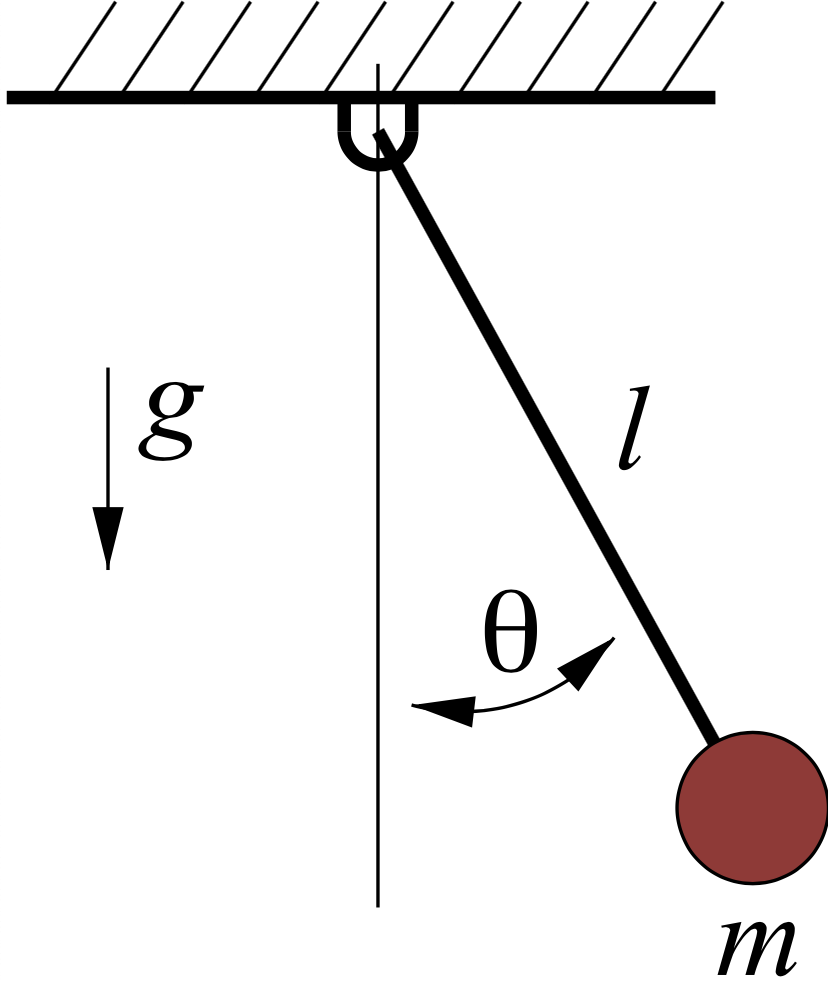
\includegraphics[width=\columnwidth]{figures/simple_pend.png}
\end{figure}
\end{columns}
\pause \pause
\begin{block}{Lyapunov theorem (sketch)}
$\dot x = f(x)$ is stable if there exists $v(x) \geq 0$ such that $\dot v(x) = \frac{\partial v}{\partial x} (x) f(x) \leq 0$
\end{block}
\end{frame}

\begin{frame}{Dynamic programming}
\begin{itemize}
\item
The state-space approach to optimal control is called \textbf{Dynamic Programming} (DP)
\item
At its core we have the \textbf{Hamilton-Jacobi-Bellman} (HJB) equation
$$
\min_{u \in U} \left\{ l(x, u) + \frac{\partial v}{\partial x} (x) f(x, u) \right\} = 0, \quad \text{for all } x
$$
recall that $v(x_0)$ is the minimum of the optimal control problem for $x(0) = x_0$
\end{itemize}
\pause
\begin{block}{$\frac{\text{Dynamic programming}}{\text{Optimal control}} = \frac{\text{Lyapunov theorem}}{\text{Stability analisis}}\ ?$ Not quite...}
\begin{itemize}
\item
In time, optimal control has similar issues to stability (we end up with hard ODEs)
\item
In state space:
\begin{itemize}
\item
HJB is a nasty nonlinear Partial Differential Equation (PDE)
\item
Lyapunov conditions ($v(x) \geq 0$, $\dot v(x) \leq 0$) are simple linear differential inequalities
\end{itemize}
\end{itemize}
\end{block}
\end{frame}

\begin{frame}{Quoting the authors}
\begin{columns}
\column{.5\textwidth}
\begin{columns}
\column{.2\columnwidth}
\begin{figure}
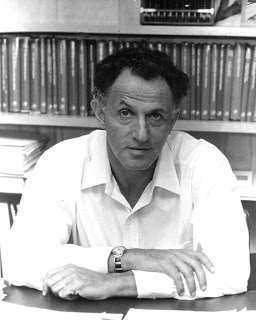
\includegraphics[width=\columnwidth]{figures/bellman.jpg}
\end{figure}
\column{.75\columnwidth}
Bellman (1957), \\ ``Dynamic Programming''
\end{columns}
\begin{figure}[h]
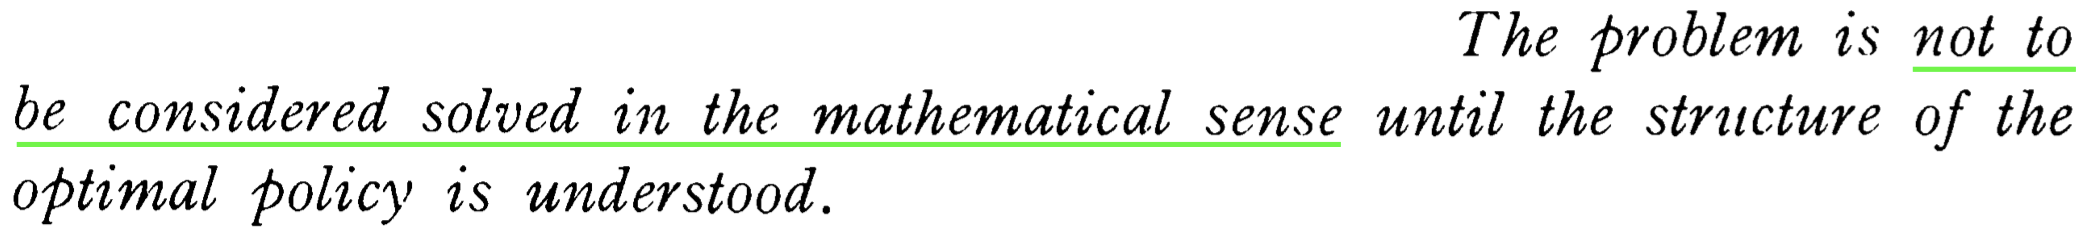
\includegraphics[width=.9\columnwidth]{figures/bellman_quote_1.png} \\
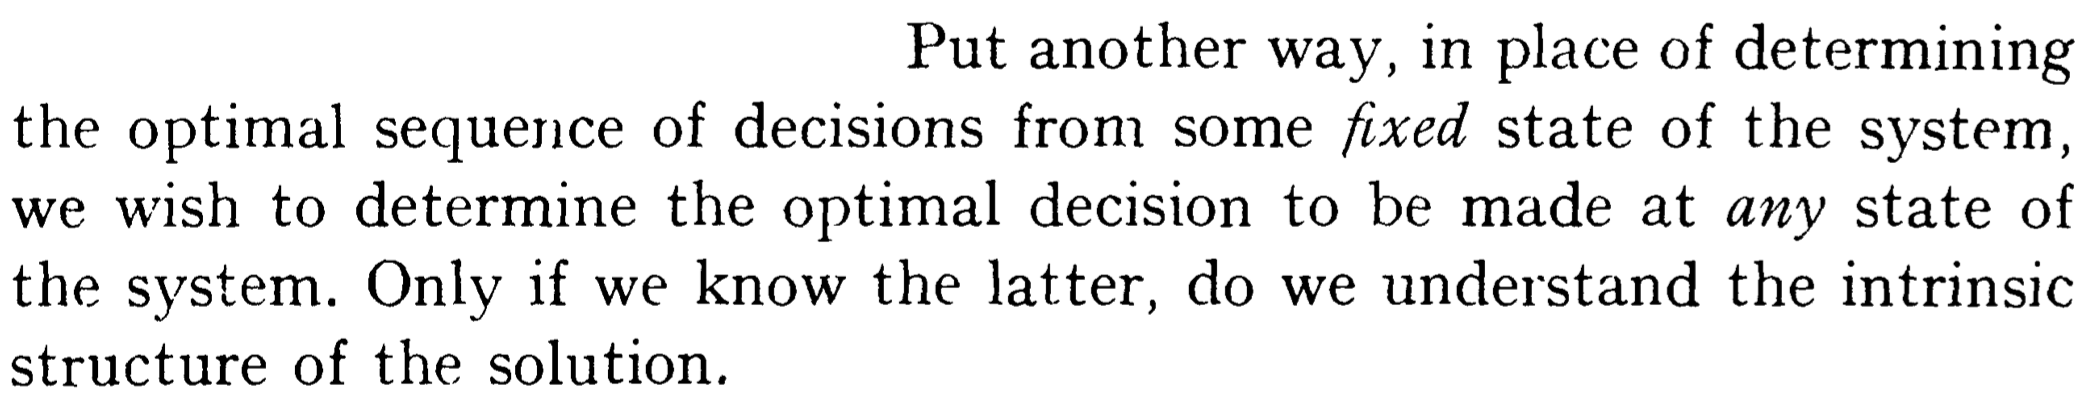
\includegraphics[width=.9\columnwidth]{figures/bellman_quote_2.png} \\
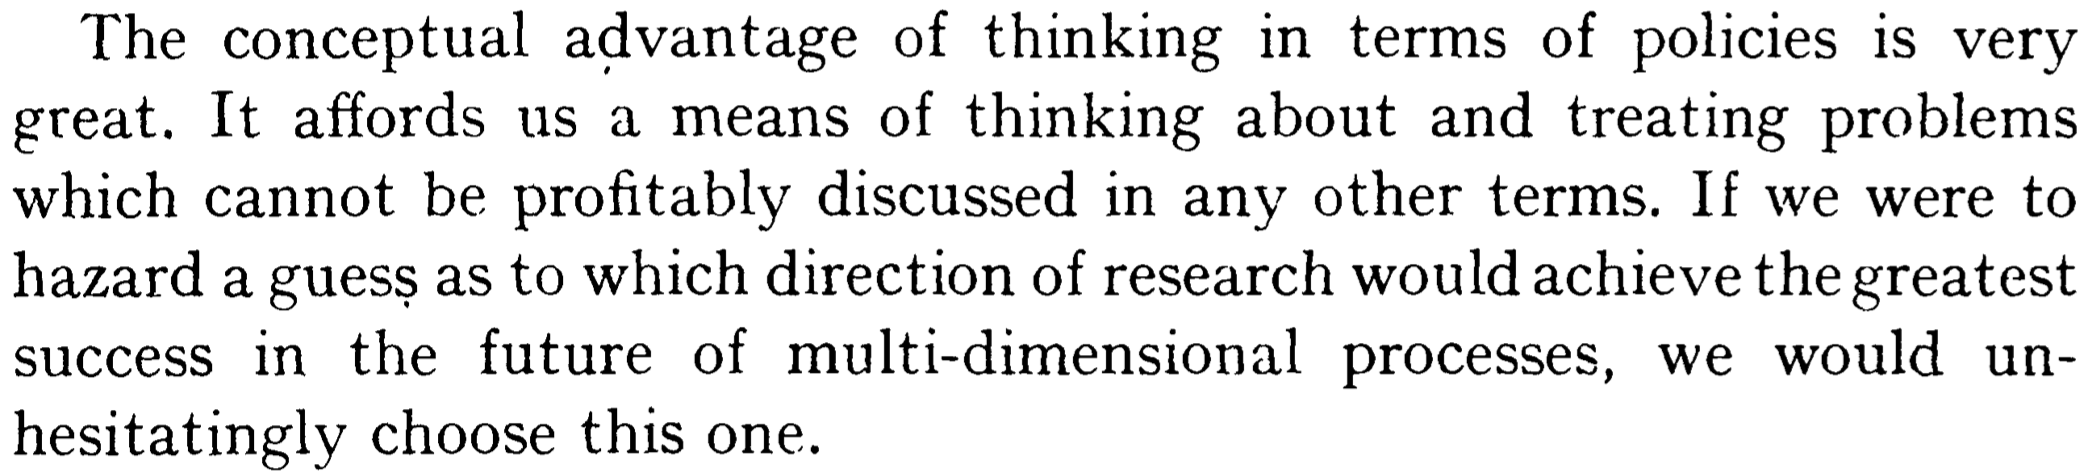
\includegraphics[width=.9\columnwidth]{figures/bellman_quote_3.png}
\end{figure}
\column{.5\textwidth}
\begin{columns}
\column{.15\columnwidth}
\begin{figure}
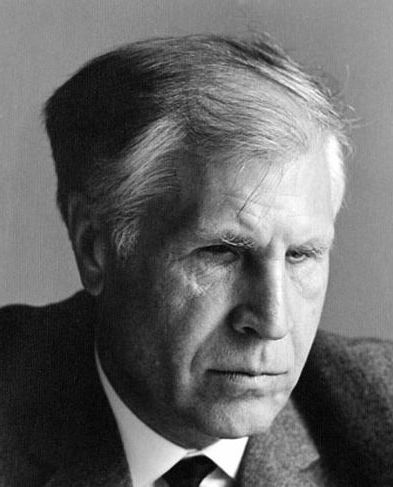
\includegraphics[width=\columnwidth]{figures/pontryagin.jpg}
\end{figure}
\column{.75\columnwidth}
Pontryagin et al. (1962), \\
``The Mathematical Theory of Optimal Processes'' 
\end{columns}

\begin{figure}[h]
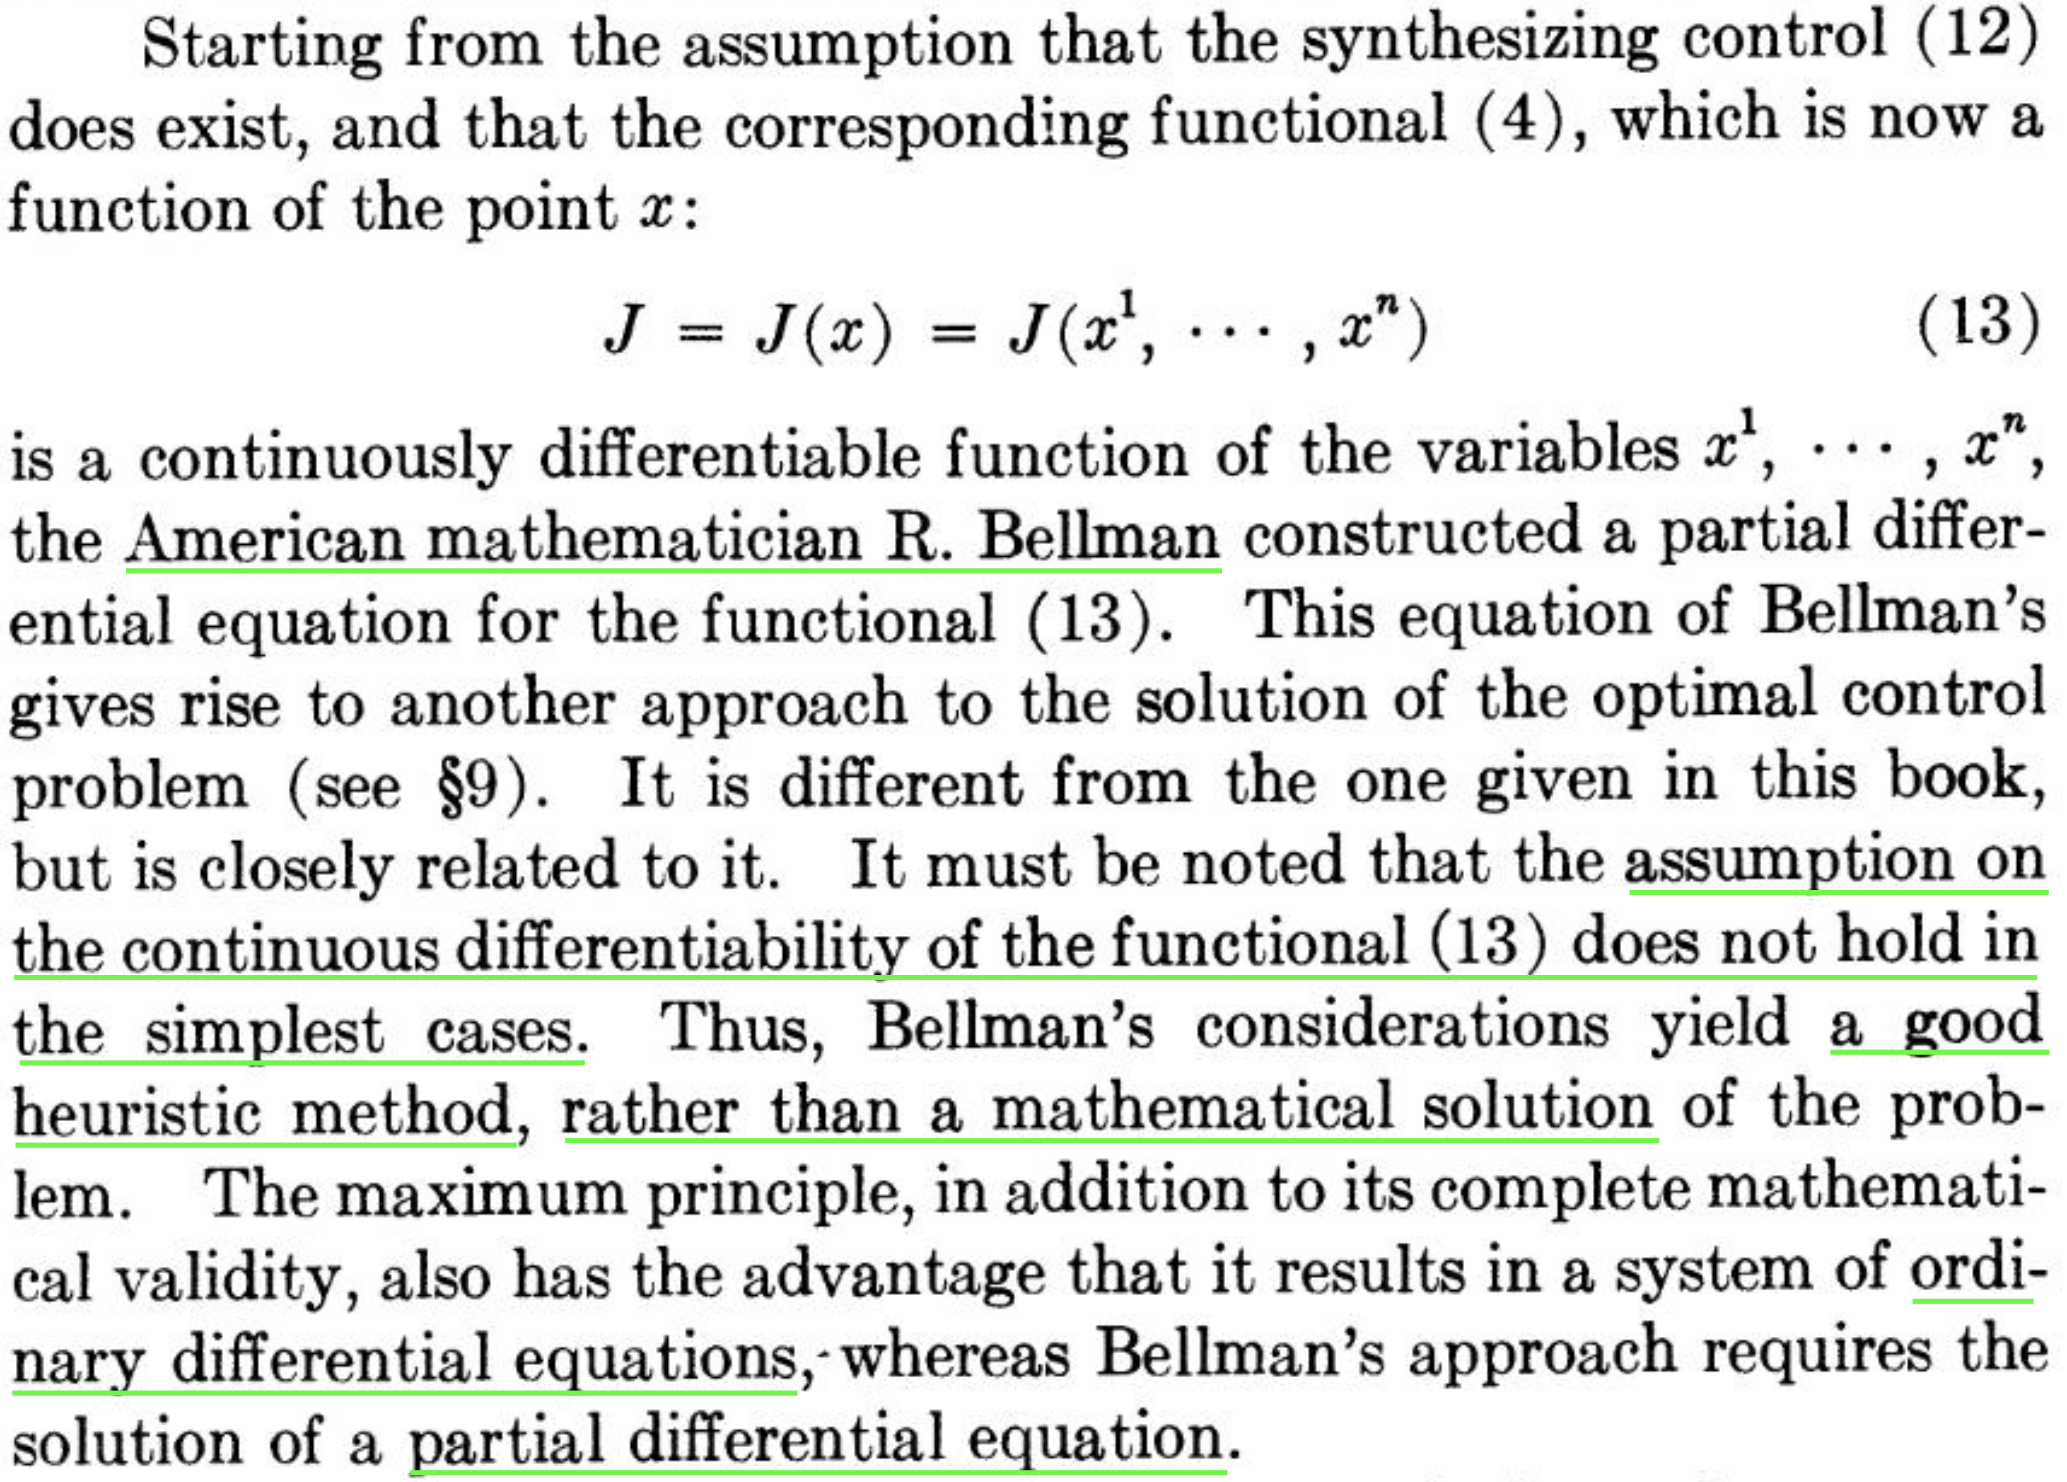
\includegraphics[width=.9\columnwidth]{figures/pontryagin_quote.png}
\end{figure}
\end{columns}
\end{frame}

\begin{frame}{Our goal today}
Use \textbf{convex optimization} to design functions in state space:
\begin{itemize}
\item
SemiDefinite Programming (SDP)
\item
Sums-of-Squares (SOS) optimization
\end{itemize}
\pause
\textbf{Two main applications}:
\begin{itemize}
\item
Design of Lyapunov functions
\begin{itemize}
\item
Not really optimal control, but of fundamental importance
\item
Convex optimization will be a game changer here
\end{itemize}
\item
Approximate dynamic programming
\begin{itemize}
\item
Convex optimization will be quite effective here
\end{itemize}
\end{itemize}
\end{frame}

\section{Convex-optimization background}
\begin{frame}
\huge
\centering
{\color{darkred} Convex-optimization background}
\end{frame}

\begin{frame}{Convex optimization recap}
\begin{columns}
\column{.5\textwidth}
Standard convex program:
\begin{align*}
\min_{x} \ &f(x) \\
\text{subject to} \ & x \in X
\end{align*}
\begin{itemize}
\item
$f$ is a convex function
\item
$X$ is a convex set
\end{itemize}
\column{.5\textwidth}
\begin{figure}
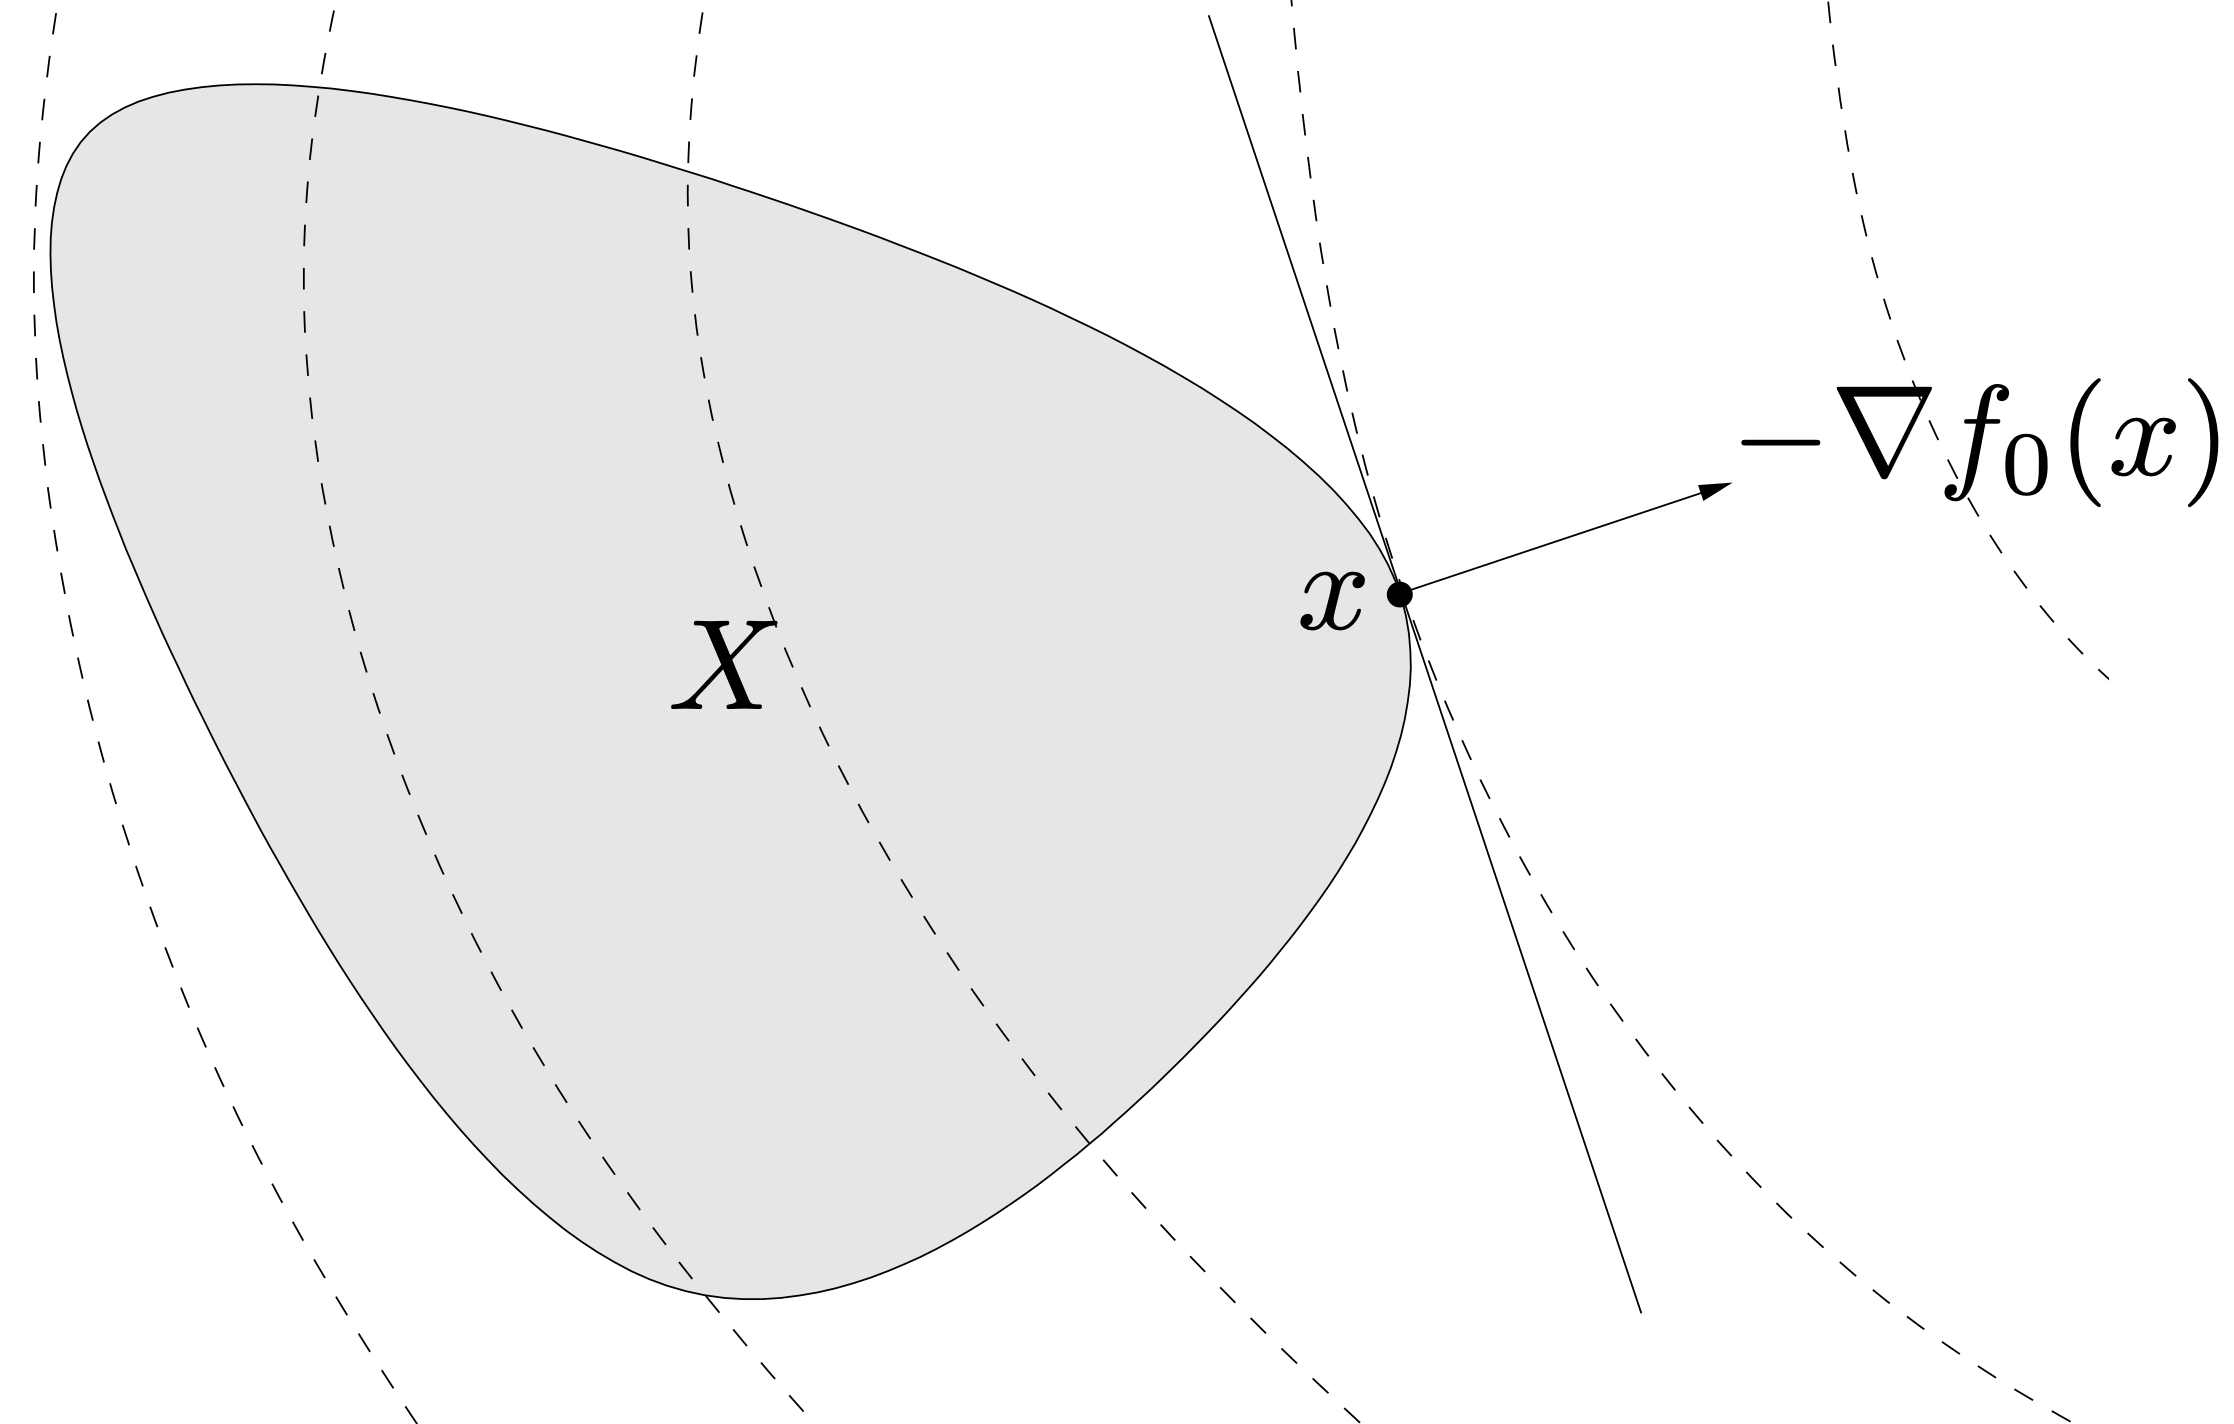
\includegraphics[width=.8\columnwidth]{figures/convex_opt.png} \\
\footnotesize Boyd, Vandenberghe - ``Convex Optimization''
\end{figure}
\end{columns}
\pause
\begin{block}{Why are we so obsessed with convex optimization?}
Every local minimum is a \textbf{global minimum}
\end{block}
\end{frame}

\begin{frame}{Proof of ``every local minimum is global''}
\begin{itemize}
\item
If $x^*$ is a local minimum, there exists $r > 0$ such that
$$
x^* = \arg \min_{x \in X} \{ f(x) : \|x - x^*\| \leq r \}
$$
\pause
\item
If $x^*$ was not a global minimum, there would exist $y \in X$ such that $f(y) < f(x^*)$
\begin{itemize}
\item
and, necessarily, $\|y - x^*\| > r$
\end{itemize}
\pause
\item
Take a point $z$ on the line connecting $x^*$ and $y$, distant $r/2$ from $x^*$:
$$
z := x^* + \theta (y - x^*) = (1 - \theta) x^* + \theta y, \quad \theta := \frac{r}{2 \|y - x^*\|}
$$
\pause
\item
By convexity of the feasible set $X$, $z \in X$
\pause
\item
By convexity of the objective,
$$
f(z) \leq (1 - \theta) f(x^*) + \theta f(y) < (1 - \theta) f(x^*) + \theta f(x^*) = f_0(x^*)
$$
which contradicts the local optimality of $x^*$
\end{itemize}
\end{frame}

\begin{frame}{A hierarchy of Convex Programs (CPs)}
\begin{columns}
\column{.7\textwidth}
\begin{itemize}
\item
Linear Programs (LPs) are the easiest
\item
SemiDefinite Programming (SDP) is a broad class of CPs that can be solved efficiently (our main tool today)
\item
Some CPs outside the class of SDP can be quite hard
\end{itemize}
\onslide<2->{
\begin{block}{What? Hard convex optimizations?? }
\begin{itemize}
\item
Optimization algorithms require to check how far a point is from being infeasible
\item
Some convex sets are very hard to describe mathematically!
\item
We'll come back to this point...
\end{itemize}
\end{block}
}
\column{.3\textwidth}
\begin{figure}
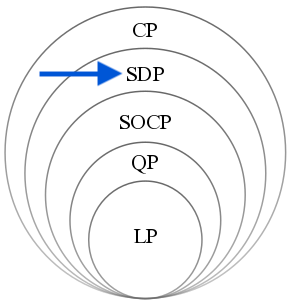
\includegraphics[width=\columnwidth]{figures/hierarchy.png}
\end{figure}
\end{columns}
\end{frame}

\begin{frame}{Definite symmetric matrices}
\begin{block}{Definition}
Equivalent definitions for a symmetric matrix $A$ to be \textbf{positive semidefinite} ($A \succeq 0$):
\begin{itemize}
\item
$x^T A x \geq 0$ for all $x$
\item
The eigenvalues $\lambda_1, \ldots, \lambda_n$ of $A$ are nonnegative
\item
There exists $L$ such that $A = L^T L$
\end{itemize}
\end{block}
\pause
Why do we care about positive semidefinite matrices?
\begin{itemize}
\item
The set $\mathbb S_n^+ := \{ (a_{11},\dots, a_{nn}) : A \succeq 0 \}$ is convex, where
$$
A = \begin{bmatrix}
a_{11} & a_{12} & \cdots & a_{1n} \\
a_{12} & a_{22} & \cdots & a_{2n} \\
\vdots & \vdots & \ddots & \vdots \\
a_{1n} & a_{2n} & \cdots & a_{nn} \\
\end{bmatrix}
$$
\end{itemize}
\end{frame}

\begin{frame}{Proof of ``$\mathbb S_n^+$ is convex''}
\begin{columns}
\column{.53\textwidth}
Just use the definition:
\begin{itemize}
\item
Assume $A_1 \succeq 0$ and $A_2 \succeq 0$
\item
Take a convex combination of  $A_1$ and $A_2$:
$$
A := \theta A_1 + (1- \theta) A_2, \quad \theta \in [0, 1]
$$
\item
Then, for all $x$,
$$x^T A x = \theta x^T A_1 x + (1- \theta) x^T A_2 x \geq 0$$
\end{itemize}
\column{.45\textwidth}
\begin{figure}
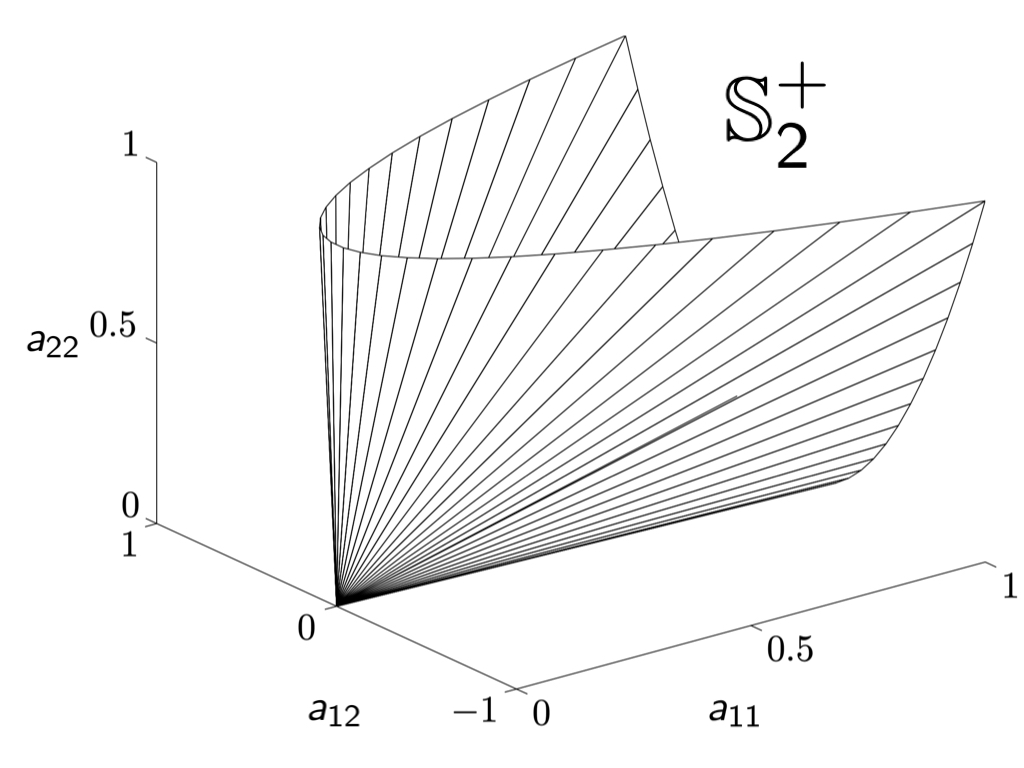
\includegraphics[width=\columnwidth]{figures/psdcone.jpeg}
\footnotesize Boyd, Vandenberghe - ``Convex Optimization''
\end{figure}
\end{columns}
\end{frame}

\begin{frame}{Semidefinite program in standard form}
\begin{columns}
	\column{.45\textwidth}
\begin{align*}
\min_{X} \ & \text{tr}(C X) \\
\text{subject to} \ & \text{tr}(A_i X) = b_i, &&  i = 1, \ldots, p \\
& X \succeq 0
\end{align*}
\column{.5\textwidth}
\begin{itemize}
\item
recall that $\text{tr}(C X) = \sum_{i,j=1}^n C_{ij} x_{ij}$, i.e., an arbitrary linear function of the entries of $A$
\item
linear objective function (convex)
\item
$p$ linear equality constraints (convex)
\item
one semideifinite constraint (convex)
\end{itemize}
\end{columns}
\pause
\begin{block}{Why can we solve SDPs efficiently?}
\begin{itemize}
\item
We need a function to tell how far is a point $(a_{11},\dots, a_{nn})$ from being infeasible
\item
Interior of the feasible set is $\{ (a_{11},\dots, a_{nn}) : \lambda_1 > 0, \ldots, \lambda_n > 0 \}$
\item
Natural candidate is $$- \sum_{i=1}^n \ln (\lambda_i) = - \ln \left( \prod_{i=1}^n \lambda_i \right) = - \ln (\det A)$$
\end{itemize}
\end{block}
\end{frame}

\section{Sums-of-squares optimization}
\begin{frame}
\huge
\centering
{\color{darkred} Sums-of-squares optimization}
\end{frame}

\begin{frame}{Nonlinear parameterization of the function space}
\begin{itemize}
\item
Ultimately, we want to use convex optimization to design functions $v(x) : \mathbb R^n \mapsto \mathbb R$
\item
\textbf{First step}: parameterize $v(x)$ with a finite number of coefficients (optimization variables)
\end{itemize}
\pause
\begin{block}{Nonnlinear parameterization}
$$
v(x) := \psi (x, \alpha)
$$
\vspace{-5mm}
\begin{itemize}
\item
$\alpha \in \mathbb R^r$ is the vector of coefficients
\item
$\psi$ is a given nonlinear scalar function
\end{itemize}
\end{block}
\pause
Say we want $v(0) = 0$:
\begin{itemize}

\item
$\psi (0, \alpha) = 0$ is a \textbf{nonnlinear equality constraint} in $\alpha$ (not convex!)
\end{itemize}
\end{frame}

\begin{frame}{Linear parameterization}
\begin{block}{Linear parameterization}
\begin{columns}
\column{.5\textwidth}
$$
v(x) := \alpha^T \psi(x)
$$
\begin{itemize}
\item
$\alpha \in \mathbb R^r$ is the vector of coefficients
\item
$\psi$ is an $r$-vector of the basis functions
\end{itemize}
\column{.35\textwidth}
\begin{figure}
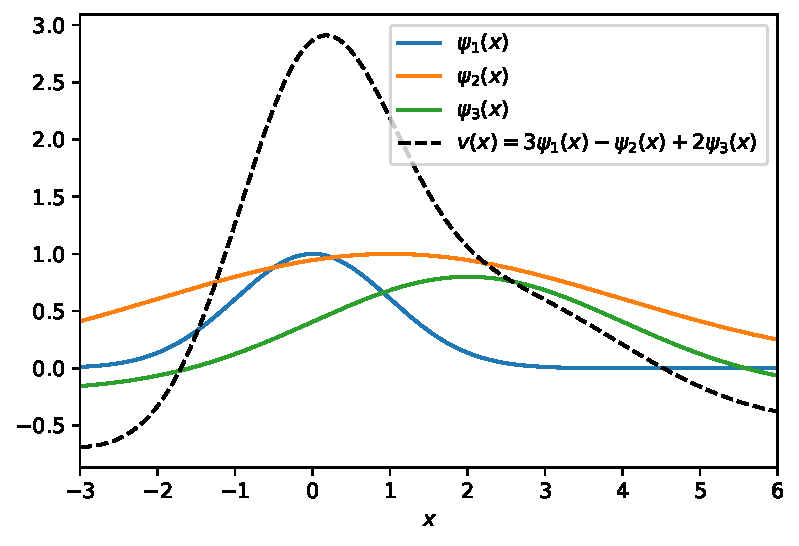
\includegraphics[width=\columnwidth]{figures/linear_parameterization.pdf}
\end{figure}
\end{columns}
\end{block}
\pause
Let's try again $v(0) = 0$:
\begin{itemize}
\item
$\alpha^T \psi(0) = 0$ is a \textbf{linear equality constraint} in $\alpha$ (convex)
\end{itemize}
\end{frame}

\begin{frame}{Other ways we might want to constrain $v(x)$?}
\begin{block}{Nonnegativity constraints}
\begin{columns}
\column{.6\textwidth}
For example, a Lyapunov function must be nonnegative
$$
v(x) := \alpha^T \psi(x) \geq 0 \text{ for all } x
$$
\column{.35\textwidth}
\begin{figure}
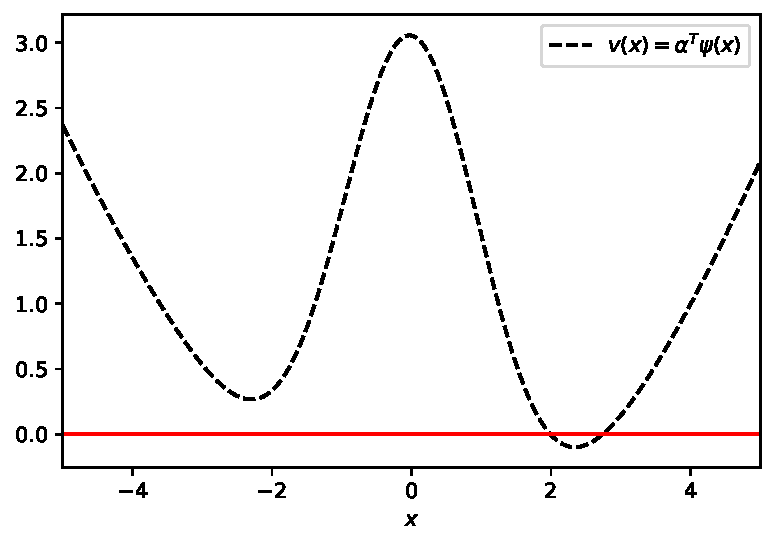
\includegraphics[width=\columnwidth]{figures/nonnegative.pdf}
\end{figure}
\end{columns}
\end{block}
\pause
Let's analyze the set
$$
\{ \alpha : \alpha^T \psi(x) \geq 0 \text{ for all } x\} \subseteq \mathbb R^r
$$
\end{frame}

\begin{frame}{Nonnegativity constraints and linear parameterizations}
\begin{block}{The set $\{ \alpha : \alpha^T \psi(x) \geq 0\}$ is convex}
\begin{itemize}
\item
Assume $\alpha_1$ is such that $v_1(x) := \alpha_1^T \psi(x) \geq 0$, and the same for $\alpha_2$
\item
Take a convex combination of $\alpha_1$ and $\alpha_2$
$$
\alpha := \theta \alpha_1 + (1 - \theta) \alpha_2, \quad \theta \in [0, 1]
$$
\item
Then $v(x) := \alpha^T \psi(x) = \theta v_1(x)  + (1 - \theta) v_2(x)  \geq 0$
\end{itemize}
\end{block}
\pause
Does this mean that optimizing over nonnegative $v(x)$ is easy?
\begin{itemize}
\item
No, in general, no
\item
Except for a few cases, for a given $\alpha$, determining if $\alpha^T \psi(x) \geq 0$ is NP-hard!
%\item
%We don't have a nice function to repel a point $\alpha$ from the boundary of the feasible set
\end{itemize}
\end{frame}

\begin{frame}{Back to the black board}
What about a parameterization that is nonnegative by construction?
\pause
\begin{block}{Sums Of Squares (SOS)}
$$
v(x) := \psi^T(x) Q \psi(x), \quad Q \succeq 0
$$
\begin{itemize}
\item
$Q$ is an $r$-by-$r$ matrix of coefficients (entries of $Q$ are our optimization variables)
\item
$\psi$ is an $r$-vector of basis functions
\end{itemize}
\end{block}
\pause
Remarks:
\begin{itemize}
\item
$v(x)= \sum_{i,j=1}^r Q_{ij}\psi_i(x) \psi_j(x)$ is still linear in $Q$
\begin{itemize}
\item
E.g., $v(0) = 0$ is a \textbf{linear constraint} on the entries of $Q$
\end{itemize}
\item
$Q \succeq 0$ is a \textbf{convex constraint}
\end{itemize}
\end{frame}

\begin{frame}{Use SOS as a constraints}
What if we want to certify that a given function $v(x)$ is nonnegative?
\pause
\begin{itemize}
\item
We can try to find a SOS decomposition $v(x) = \psi^T(x) Q \psi(x)$, with $Q \succeq 0$
\item
The issue is how to pick $\psi(x)$...
\end{itemize}
\pause
\begin{block}{Example}
\begin{columns}
\column{.7\textwidth}
\begin{itemize}
\item
Consider $v(x) = \frac{1}{\sqrt{1 + x^2}}$
\item
Nonnegative for all $x$
\item
I don't quite know how to pick $\psi(x)$ here
\end{itemize}
\column{.25\textwidth}
\begin{figure}
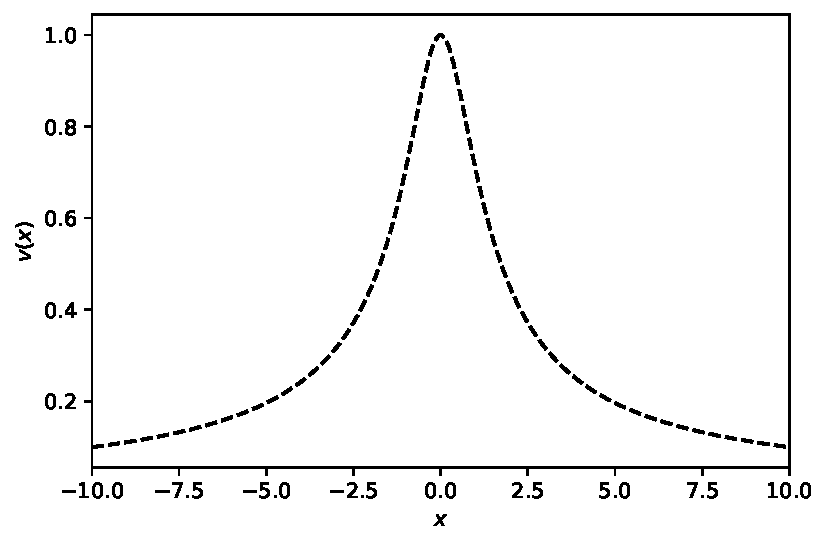
\includegraphics[width=\columnwidth]{figures/imq.pdf}
\end{figure}
\end{columns}
\end{block}
\pause
Can you think of any class of functions for which this approach might work?
\end{frame}

\begin{frame}{SOS polynomials}
\begin{block}{Example}
\begin{itemize}
\item
Given $v(x) = 2 - 2 x + 3 x^2 + 2 x^3 + x^4$, we want $\psi(x)$ such that $v(x) = \psi^T(x) Q \psi(x)$
\item
We can just pick $\psi(x) := (1, x, x^2)$
\item
Then, we look for $Q \succeq 0$ such that
\vspace{-5mm}
$$
2 - 2 x + 3 x^2 + 2 x^3 + x^4 =
\begin{bmatrix} 1 \\ x \\ x^2 \end{bmatrix}^T
\begin{bmatrix} Q_{11} & Q_{12} & Q_{13} \\ Q_{12} & Q_{22} & Q_{23} \\ Q_{13} & Q_{23} & Q_{33} \end{bmatrix}
\begin{bmatrix} 1 \\ x \\ x^2 \end{bmatrix}
$$
\item
Comparing the coefficients we get \textbf{linear constraints} on $Q$, e.g., $Q_{11} = 2$
\end{itemize}
\end{block}
\pause
\begin{itemize}
\item
For $v(x)$ \textbf{polynomial} of degree $2d$, we fill $\psi(x)$ with all the \textbf{monomials} up to degree $d$
\pause
\item
This works even if the coefficients of $v$ are (linear functions of) optimization variables
\pause
\item
Other classes of functions could work, polynomials have many properties
\end{itemize}
\end{frame}

\begin{frame}{The power of SOS optimization \href{https://colab.research.google.com/github/TobiaMarcucci/optimal_control_pisa/blob/master/demos/six_hump_camel.ipynb}{\beamergotobutton{Try this in Drake}}}
\begin{columns}
\column{.7\textwidth}
Minimize the six-hump-camel function
$$
\min_x p(x) = 4 x_1^2 + x_1 x_2 - 4 x_2^2 - 2.1 x_1^4 + 4 x_2^4 + x_1^6 / 3
$$
\onslide<2->{
\begin{itemize}
\item
Write it as
\begin{align*}
\max_{ \lambda, Q} \ & \lambda \\
\text{subject to} \ &  p(x) - \lambda \text{ is SOS}
\end{align*}
where ``is SOS'' means ``equal to a SOS polynomial in $x$ parameterized by $Q$''
\end{itemize}
}
\column{.3\textwidth}
\vspace{-5mm}
\begin{figure}
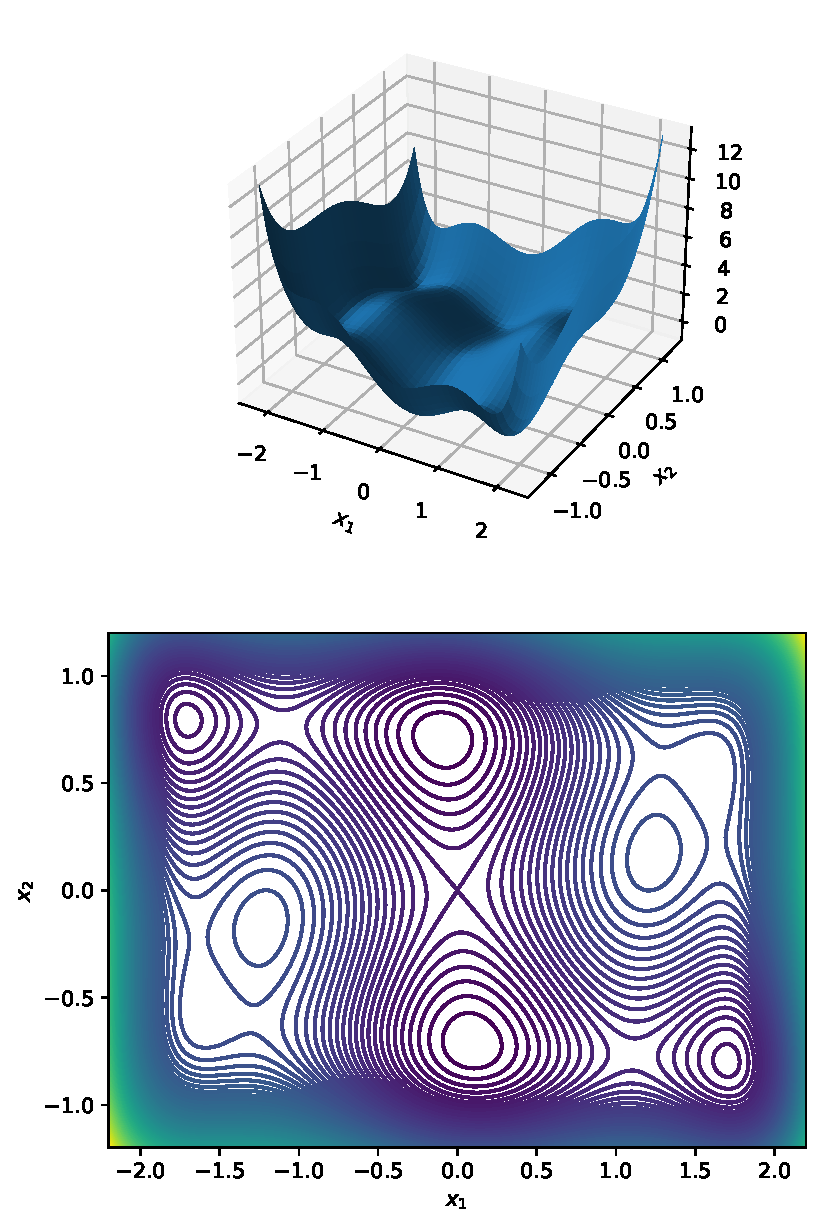
\includegraphics[width=\columnwidth]{figures/camel.pdf}
\end{figure}
\end{columns}
\end{frame}

\begin{frame}{Did we just solve global optimization over polynomials?}
\begin{columns}
\column{.6\textwidth}
Not all the nonnegative polynomials are SOS!
\begin{itemize}
\item
Hilbert in 1888\footnotemark showed that ``SOS = nonnegative'' only in 3 cases\footnotemark:
\begin{itemize}
\item
Univariate polynomials (1 variable)
\item
Quadratic polynomials (degree 2)
\item
Bivariate quartics (2 variables, degree 4)
\end{itemize}
\onslide<2->{
\item
Famous counterexample by Motzkin
$$x_1^4 x_2^2 + x_1^2 x_2^4 + 1 - 3 x_1^2 x_2 ^2$$
\item
Counterexamples are ``rare enough that people give names to them''
}
\end{itemize}
\column{.25\textwidth}
\begin{figure}
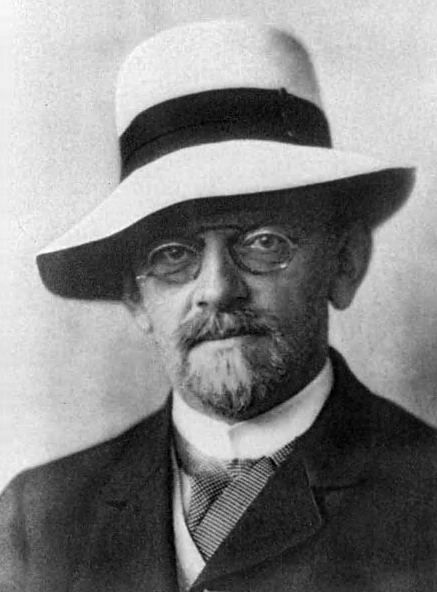
\includegraphics[width=.4\columnwidth]{figures/hilbert.jpg}
\onslide<2->{
\vspace{-10mm}
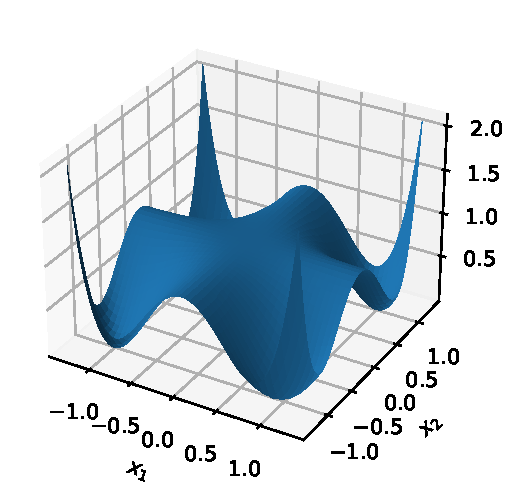
\includegraphics[width=\columnwidth]{figures/motzkin.pdf}
}
\end{figure}
\end{columns}
\footnotetext[1]{Hilbert - ``Ueber die Darstellung definiter Formen als Summe von Formenquadraten''}
\footnotetext[2]{See also \href{https://en.wikipedia.org/wiki/Hilbert\%27s_seventeenth_problem}{{\color{blue}Hilbert's 17th problem}}}
\end{frame}

\begin{frame}{Constrained SOS: the S-procedure}
\begin{itemize}
\item
To constrain the polynomial $v(x)$ to be nonnegative over the set
$$
\{ x :  g(x) = 0 \}
$$
with $g(x)$ polynomial, we can add a new polynomial $\lambda(x)$ and write
$$
v(x) + \lambda(x) g(x) \text{ is SOS}
$$
\end{itemize}
\pause
\begin{columns}
\column{.65\textwidth}
\begin{itemize}
\item
Similarly, for the set
$$
\{ x :  g(x) \leq 0 \}
$$
we can add a new SOS polynomial $\lambda(x)$ and write
$$
v(x) + \lambda(x) g(x) \text{ is SOS}
$$
\end{itemize}
\column{.3\textwidth}
\begin{figure}
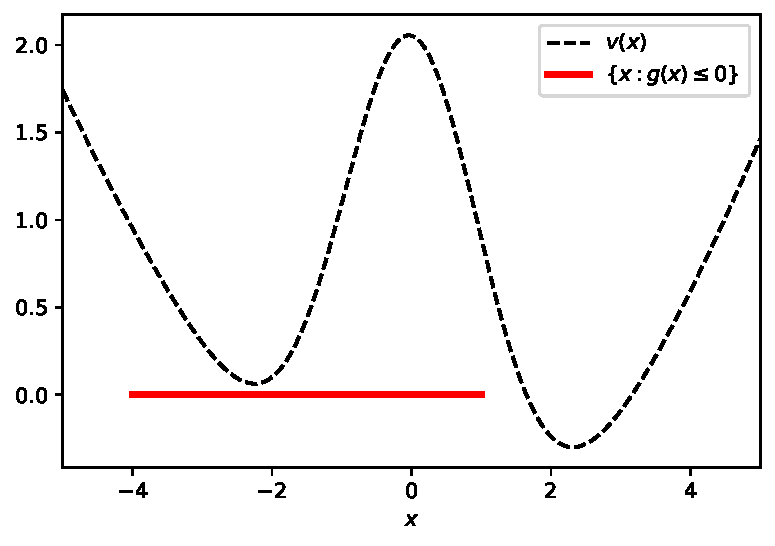
\includegraphics[width=\columnwidth]{figures/s_procedure.pdf}
\end{figure}
\end{columns}
\end{frame}

\section{Design of Lyapunov functions}
\begin{frame}
\huge
\centering
{\color{darkred} Design of Lyapunov functions}
\end{frame}

\begin{frame}{Recap on Lyapunov stability}
\begin{columns}
\column{.55\textwidth}
The equilibrium $x=0$ for the system $\dot x = f(x)$ is:
\begin{itemize}
\item
\textbf{stable} if, for all $\varepsilon > 0$, there exists $\delta > 0$ such that
$$
\|x(0)\| < \delta \Rightarrow \|x(t)\| < \varepsilon \text{ for all }  t \geq 0
$$
\item<2->
\textbf{asymptotically stable} if it is stable, and $\lim_{t \rightarrow \infty} \| x(t)\| = 0$
\end{itemize}
\column{.4\textwidth}
\begin{figure}
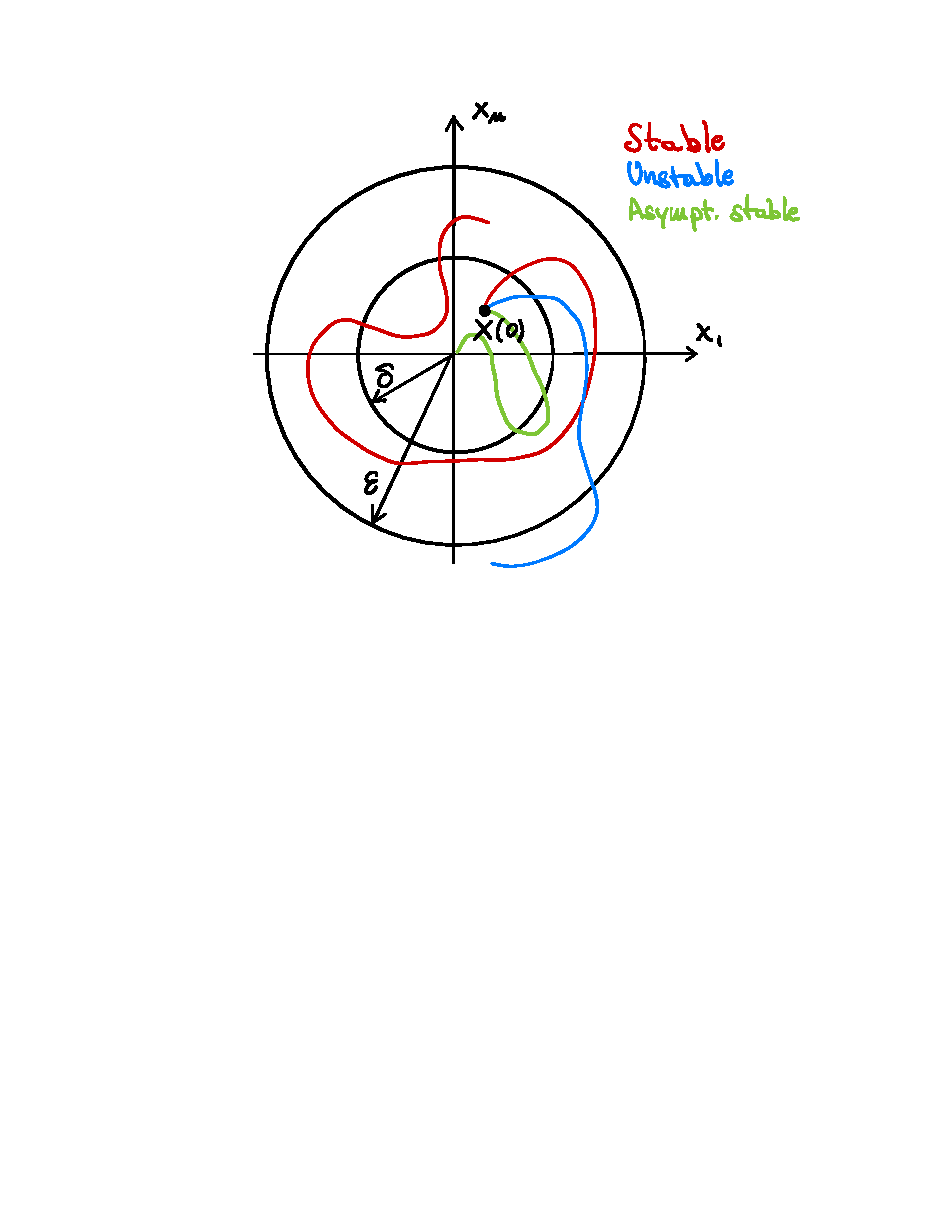
\includegraphics[width=\columnwidth]{figures/stability.pdf}
\end{figure}
\end{columns}
\end{frame}

\begin{frame}{Recap on Lyapunov direct method}
\begin{columns}
\column{.6\textwidth}
The equilibrium $x=0$ for the system $\dot x = f(x)$ is:
\begin{itemize}
\item
\textbf{stable} iff there exists $v(x)$ such that
$$
v(0) = 0, \quad v(x) > 0 \text{ for all } x \neq 0,
$$
and
$$
\dot v(x) = \frac{\partial v}{\partial x}(x) f(x) \leq 0 \text{ for all }  x \neq 0
$$
\item<2->
\textbf{asymptotically stable} iff
$$
\dot v(x) < 0 \text{ for all }  x \neq 0
$$
\end{itemize}
\column{.4\textwidth}
\begin{figure}
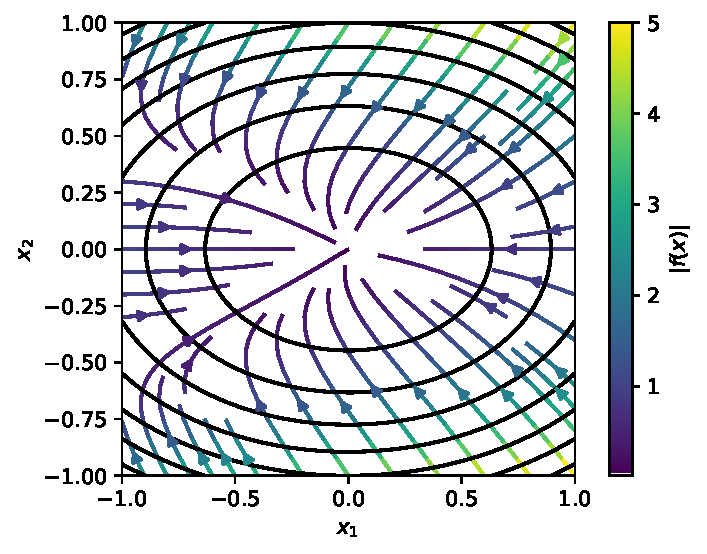
\includegraphics[width=\columnwidth]{figures/lyapunov_poly.pdf}
\end{figure}
\end{columns}
\end{frame}


\begin{frame}{Design of Lyapunov functions via SOS}
SOS parameterization of the Lyapunov function
$$
v(x) = \psi^T(x) Q \psi(x), \quad Q \succeq 0
$$
\pause
\vspace{-5mm}
\begin{block}{We choose to work with polynomials}
The vector $\psi(x)$ contains all the monomials up to a certain degree
\pause
\begin{itemize}
\item
Works in the linear case $f(x) = A x$ (there always exists $v(x) = x^T P x$)
\pause
\item
If $f(x)$ is polynomial, then
$$
\dot v(x) = \frac{\partial v}{\partial x}(x) f(x)
$$
is also polynomial, and its coefficients are linear in $Q$
\pause
\item
If $f(x)$ is not polynomial we can use, e.g., Taylor approximation
\end{itemize}
\end{block}
\end{frame}

\begin{frame}{Design of Lyapunov functions via SOS
\href{https://colab.research.google.com/github/TobiaMarcucci/optimal_control_pisa/blob/master/demos/lyapunov_poly.ipynb}{\beamergotobutton{Try this in Drake}}}
\begin{columns}
\column{.6\textwidth}
\begin{block}{The overall SOS program}
$$
\text{find } v(x) \text{ SOS} : - \frac{\partial v}{\partial x}(x) f(x) \text{ is SOS}
$$
\end{block}
\onslide<2->{
Miscellaneous:
\begin{itemize}
\item
To rule out the trivial solution $v(x) = 0$ we can require $v(1) = 1$
\item
Complexity is polynomial in the number of states $x$, but exponential in the degree of $v$
\item
Another ``leak'': not all the stable polynomial systems admit a polynomial Lyapunov function\footnotemark
\end{itemize}
}
\column{.2\textwidth}
\begin{figure}
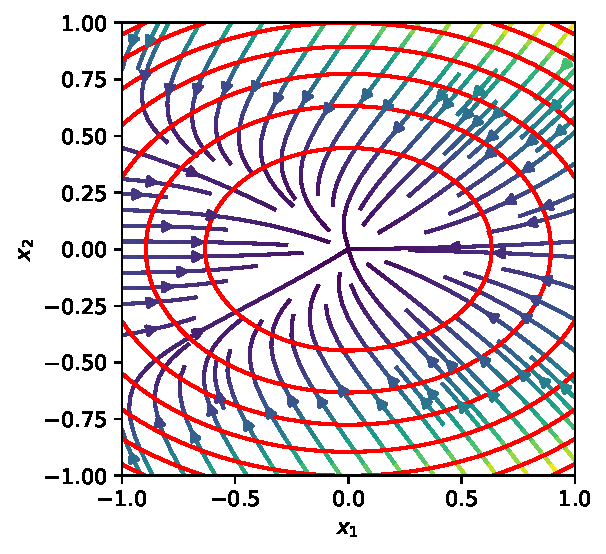
\includegraphics[width=\columnwidth]{figures/lyapunov_poly_1.pdf}
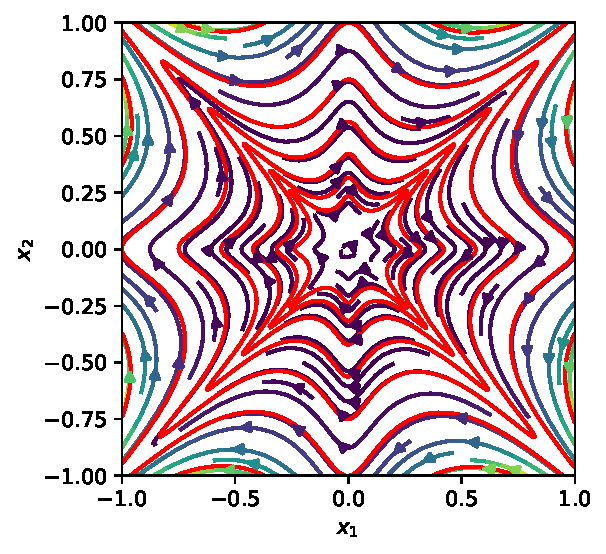
\includegraphics[width=\columnwidth]{figures/lyapunov_poly_2.pdf}
\end{figure}
\end{columns}
\footnotetext[1]{Ahmadi, Krstic, Parrilo - ``A Globally Asymptotically Stable Polynomial Vector Field with no Polynomial Lyapunov Function''}
\end{frame}

\begin{frame}{Verification of non-polynomial systems via SOS
\href{https://colab.research.google.com/github/TobiaMarcucci/optimal_control_pisa/blob/master/demos/lyapunov_pendulum.ipynb}{\beamergotobutton{Try this in Drake}}}
\begin{columns}
\column{.65\textwidth}
\begin{itemize}
\item
Some non-polynomial systems can be verified exactly using SOS\footnotemark
$$
\dot x_1 = x_2, \quad
\dot x_2 = - x_2 - \sin(x_1)
$$
\item<2->
Introduce auxiliary variables $s = \sin(x_1)$, $c = \cos(x_1)$
\item<3->
Substitute to get the polynomial system
$$
\dot s = c x_2, \quad
\dot c = - s x_2, \quad
\dot x_2 = - x_2 - s
$$
subject to the polynomial constraint $s^2 + c^2 = 1$
\end{itemize}
\column{.3\textwidth}
\begin{figure}[h]
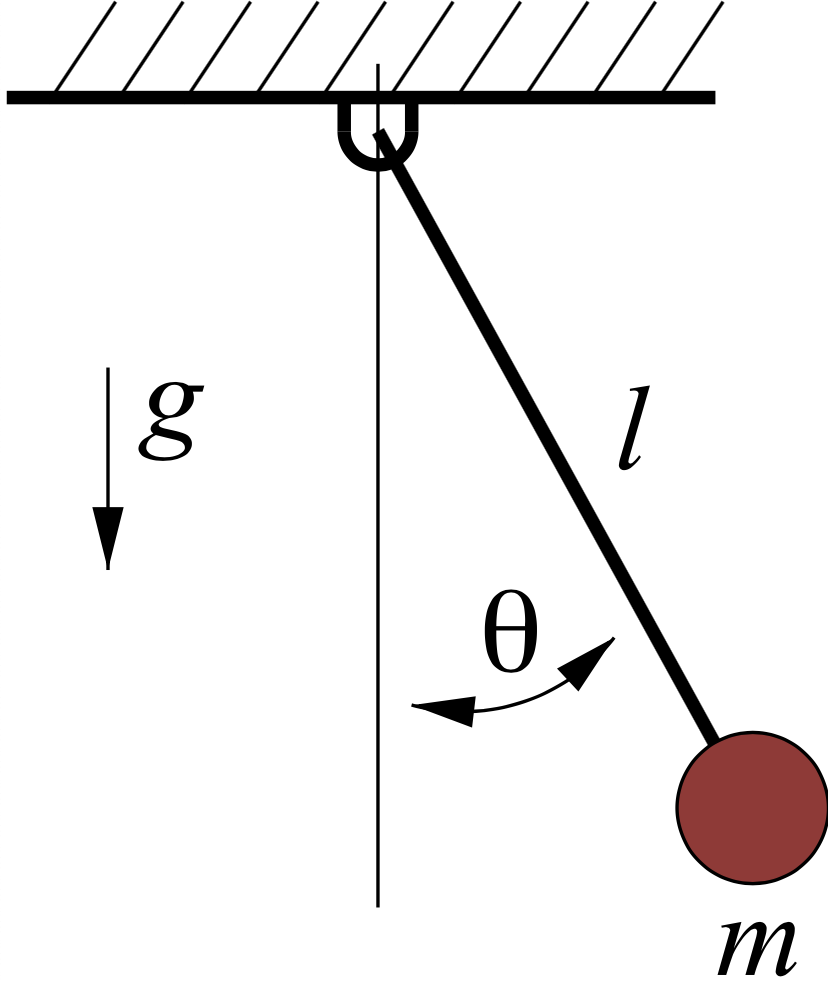
\includegraphics[width=.5\columnwidth]{figures/simple_pend.png} \\
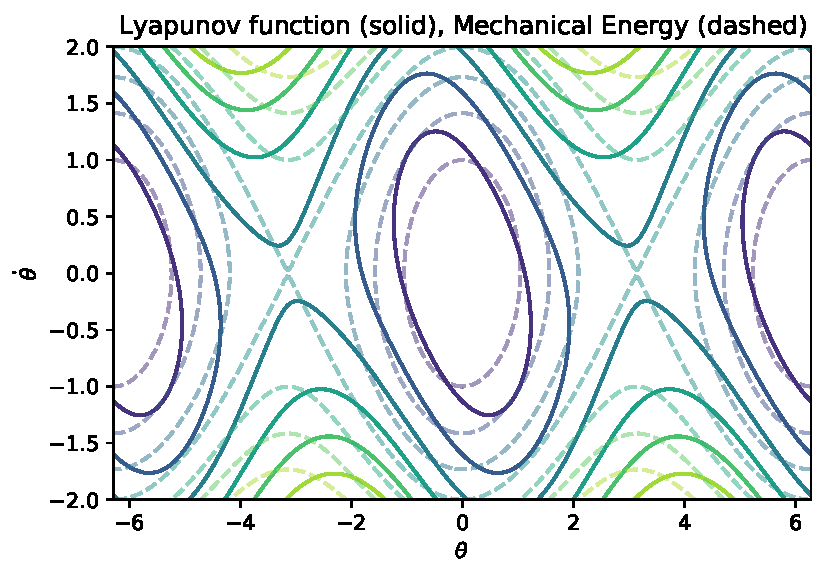
\includegraphics[width=\columnwidth]{figures/lyapunov_pendulum.pdf}
\end{figure}
\end{columns}
\footnotetext[1]{See also Papachristodoulou, Prajna - ``Analysis of Non-polynomial Systems using the Sum of Squares Decomposition''}
\end{frame}

\begin{frame}{Approximation of region of attraction via SOS
\href{https://colab.research.google.com/github/RussTedrake/underactuated/blob/master/examples/lyapunov.ipynb}{\beamergotobutton{Try this in Drake}}}
Time-reversed Van der Pol oscillator
\begin{align*}
\dot x_1 &= - x_2 \\
\dot x_2 &= x_1 + (x_1^2 - 1) x_2
\end{align*}
\vspace{-5mm}
\begin{columns}
\column{.45\textwidth}
\begin{block}{Maximize volume of level set}
\begin{figure}
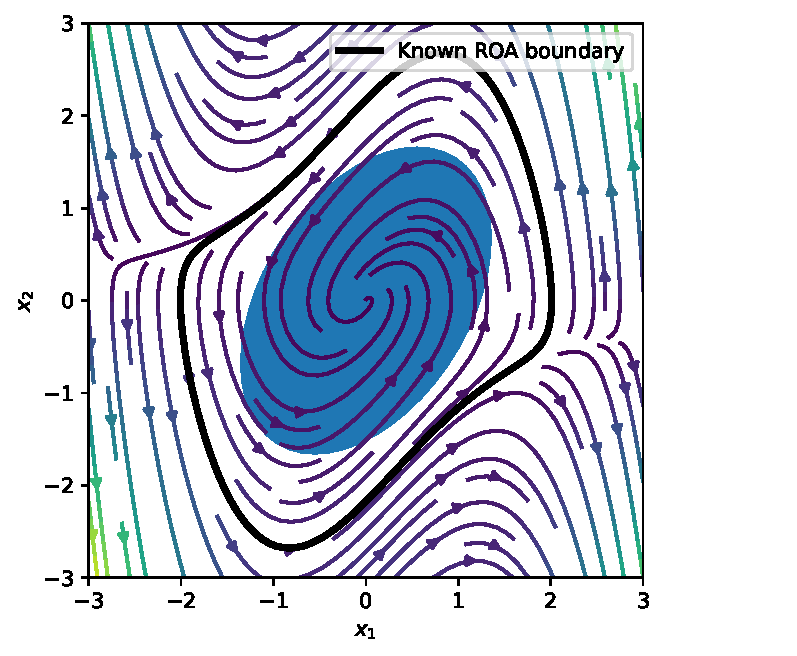
\includegraphics[width=.6\columnwidth]{figures/van_der_pol_roa_quadratic.pdf}
\end{figure}
\end{block}
\column{.45\textwidth}
\begin{block}{Alternate maximization of level set and reshape Lyapunov function}
\begin{figure}
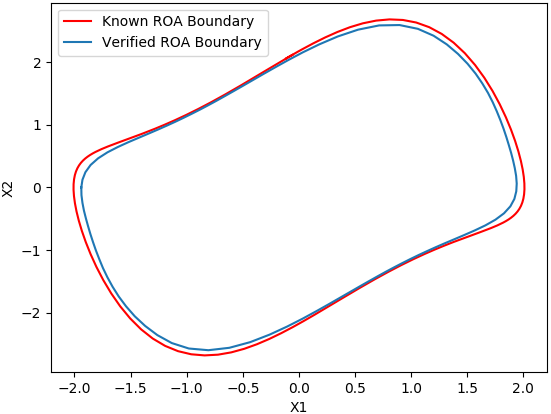
\includegraphics[width=.7\columnwidth]{figures/van_der_pol_roa.png}
\end{figure}
\end{block}
\end{columns}
\end{frame}

\begin{frame}{SOS for control-Lyapunov function?}
We can't do control synthesis with Lyapunov and SOS:
\begin{itemize}
\item
SOS Lyapunov function $v(x)$ 
\item
Linear parameterization for $u(x)$
\item
For simplicity, let the system be control-affine
$$
\dot x = f(x) + G(x) u
$$
\pause
\item
Lyapunov condition is
$$
- \frac{\partial v}{\partial x}(x) [f(x) + G(x) u(x)] \text{ is SOS}
$$
\item
Multiplication of $\frac{\partial v}{\partial x}$ and $u$ leads to \textbf{nonlinear equality constraints}
\end{itemize}
\end{frame}

\section{Approximate dynamic programming}
\begin{frame}
\huge
\centering
{\color{darkred} Approximate dynamic programming}
\end{frame}

\begin{frame}{Hamilton-Jacobi-Bellman (HJB) equation}
How to arrive to the HJB equation
$$
\min_{u \in U} \left\{ l(x, u) + \frac{\partial v}{\partial x} (x) f(x, u) \right\} = 0, \quad \text{for all } x
$$
from the Optimal Control Problem (OCP)
\begin{align*}
v(x_0) := \min_{u, x} \ &\int_0^\infty l(x(t), u(t)) dt \\
\text{subject to} \ & x(0) = x_0 \\
& \dot x(t) = f(x(t), u(t)), &&  \text{for all }t \in [0, \infty) \\
& u(t) \in U, &&  \text{for all }t \in [0, \infty)
\end{align*}
\end{frame}

\begin{frame}{HJB: informal derivation}
First order approximation with time step $h$:
\begin{itemize}
\item
Cost function
$$
\int_0^\infty l(x(t), u(t)) dt
\approx
h \sum_{k=0}^\infty l(x(hk), u(hk))
$$
\vspace{-3mm}
\item
Dynamics
$$
x(t+h) \approx x(t) + h f(x(t), u(t))
$$
\pause
\vspace{-3mm}
\item
Calling $x_k := x(hk)$ and $u_k := u(hk)$, we get
\begin{align*}
v(x_0) := \min_{u, x} \ &h \sum_{k=0}^\infty l(x_k, u_k) \\
\text{subject to} \ & x_0 \text{ given} \\
& x_{k+1} = x_k + h f(x_k, u_k), &&  k = 0, \ldots, \infty \\
& u_k \in U, &&  k = 0, \ldots, \infty
\end{align*}
\end{itemize}
\end{frame}

\begin{frame}{HJB: informal derivation}
\begin{columns}
\column{.7\textwidth}
The dynamic-programming principle:
\begin{itemize}
\item
Assume $\mathbf x_0 = (x_0, x_1, x_2, x_3, \ldots)$ is the optimal trajectory from $x_0$ to the origin
\item<2->
Because of the infinite horizon, the optimal trajectory $\mathbf x_1$ from $x_1$ to the origin must be
$(x_1, x_2, x_3, \ldots)$
\begin{itemize}
\item
Otherwise $(x_0, \mathbf x_1)$ would be better than $\mathbf x_0$ (contradiction)
\end{itemize}
\item<3->
If we were to know the cost-to-go $v(x_1)$ from $x_1$, then we could just solve a one-step problem
\begin{align*}
v(x_0) & = \min_{u_0 \in U} \{ h l(x_0, u_0) + v(x_1) \} \\
& = \min_{u_0 \in U} \{ h l(x_0, u_0) + v(x_0 + h f(x_0, u_0)) \} \\
\end{align*}
\end{itemize}
\column{.3\textwidth}
\vspace{-5mm}
\begin{figure}
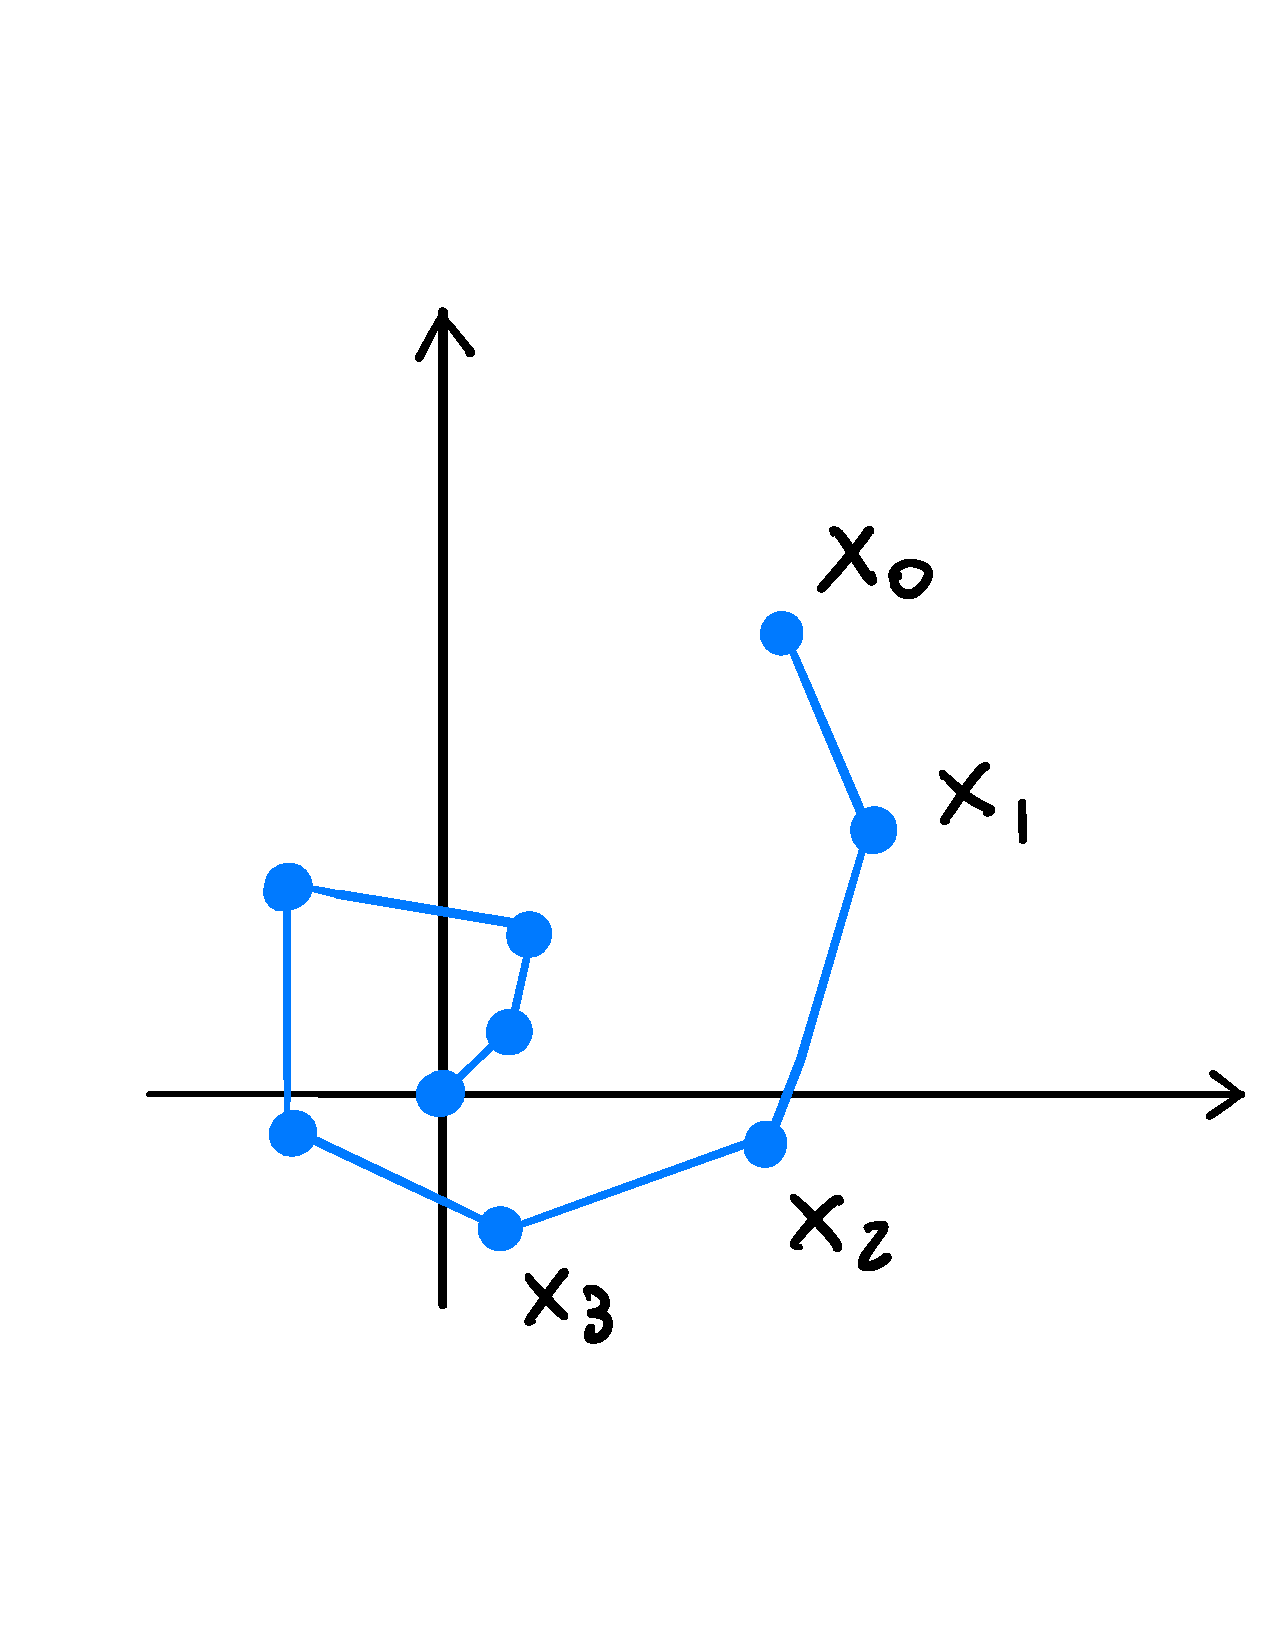
\includegraphics[width=\columnwidth]{figures/dp_principle.pdf}
\end{figure}
\end{columns}
\end{frame}

\begin{frame}{HJB: informal derivation}
\begin{itemize}
\item
If $h$ is very small,
$$
v(x_0 + h f(x_0, u_0)) \approx v(x_0) + h \frac{\partial v}{\partial x} (x_0) f(x_0, u_0)
$$
\pause
\vspace{-5mm}
\item
Substituting
$$
v(x_0) = \min_{u_0 \in U} \left\{ h l(x_0, u_0) +  v(x_0) + h \frac{\partial v}{\partial x} (x_0) f(x_0, u_0) \right\}
$$
\pause
\item
Simplifying $v(x_0)$ and dividing by $h$
$$
0 = \min_{u_0 \in U} \left\{ l(x_0, u_0) + \frac{\partial v}{\partial x} (x_0) f(x_0, u_0) \right\}
$$
\end{itemize}
\pause
\begin{block}{Observations}
\begin{itemize}
\item
If we know the value function $v(x)$, the optimal controller $u(x)$ is the argmin of the HJB
\pause
\item
Why ``informal''? (Remember the bang bang controller)
\end{itemize}
\end{block}
\end{frame}

\begin{frame}{Solving the HJB
\href{https://mybinder.org/v2/gh/RussTedrake/underactuated/master?filepath=examples\%2Fdouble\_integrator\%2Fvalue\_iteration.ipynb}{\beamergotobutton{Try this in Drake}}}
The HJB equation is a nonnlinear PDE
\begin{itemize}
\item
Analytic solutions only in a few special cases (LQR)
\item
``Exact'' numerical solution is very hard:
\begin{itemize}
\item
mainly variants of the \textbf{Value-Iteration (VI) algorithm}
\item
require discretization of the state and control space
\end{itemize}
\end{itemize}
\pause
\begin{block}{Bang-bang control of the double integrator via VI}
\begin{figure}
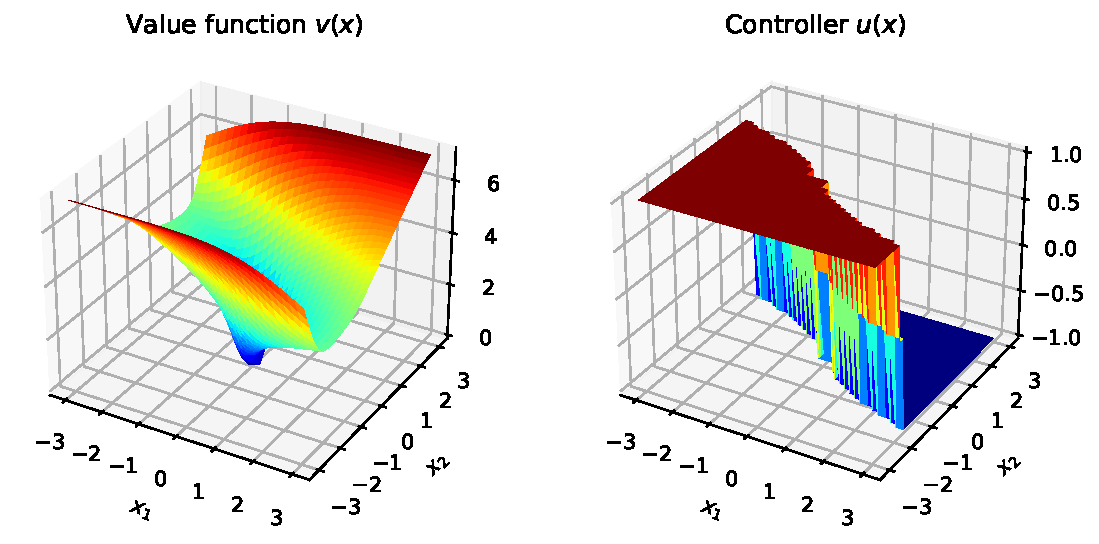
\includegraphics[width=.5\columnwidth]{figures/value_iteration.pdf}
\end{figure}
\end{block}
\end{frame}

\begin{frame}{Solving the HJB approximately}
Can we still find approximate solutions of the HJB that are ``good enough''?
\begin{block}{``One side of the HJB equation is convex''}
$$
\min_{u \in U} \left\{ l(x, u) + \frac{\partial v}{\partial x} (x) f(x, u) \right\} \geq 0, \quad \text{for all } x
$$
is equivalent to the so-called \textbf{Bellman inequality}
$$
l(x, u) + \frac{\partial v}{\partial x} (x) f(x, u) \geq 0, \quad \text{for all } x \text{ and } u \in U
$$
\vspace{-5mm}
\begin{itemize}
\item
We can relax this condition via SOS!
\end{itemize}
\end{block}
\end{frame}



\begin{frame}{Bellman inequality}
What do we loose by enforcing only one side of the HJB?
\pause
\begin{itemize}
\item
Let $x(t)$ and $u(t)$ be the optimal trajectory and control from $x(0)$
\pause
\item
Integrate the Bellman inequality along this optimal trajectory
\begin{align*}
0 & \leq \int_0^\infty \left[ l(x(t), u(t)) + \frac{\partial v}{\partial x} (x(t)) f(x(t), u(t)) \right] dt \\
& = \int_0^\infty l(x(t), u(t)) dt + \int_0^\infty \dot v(x(t)) dt \\
& = \int_0^\infty l(x(t), u(t)) dt + v(x(\infty)) - v(x(0))
\end{align*}
\pause
\item
Assume $v(0) = 0$, then $v(x)$ lower bounds the optimal value function
$$
v(x(0)) \leq \int_0^\infty l(x(t), u(t)) dt
$$
\end{itemize}
\end{frame}

\begin{frame}{SOS for approximate dynamic programming}
\begin{align*}
\max_v \ &\int_X v(x) dx \\
\text{subject to} \ & l(x, u) + \frac{\partial v}{\partial x} (x) f(x, u) \text{ is SOS for all } x \text{ and } u \in U \\
& v(0) = 0
\end{align*}
\vspace{-5mm}
\begin{block}{Interpretation}
\begin{itemize}
\item
Constraints ensure that $v(x)$ lower bounds the value function
\item
Objective ``pushes up'' $v(x)$ over the set $X$ (note that the objective is linear in $Q$)
\item
As the degree of $v(x)$ increases, we get a better and better approximation of the value function over the set $X$
\end{itemize}
\end{block}
\end{frame}

\begin{frame}{Toy approximate-DP problem
\href{https://colab.research.google.com/github/TobiaMarcucci/optimal_control_pisa/blob/master/demos/approximate_dp_scalar.ipynb}{\beamergotobutton{Try this in Drake}}}
\begin{columns}
	\column{.5\textwidth}
\begin{itemize}
	\item
	Scalar dynamics $f(x, u)= x - 4 x^3 + u$
	\item
	Quadratic running cost $l(x, u) = x^2 + u^2$
	\item
	Control limits $u \in U = [-1, 1]$
	\item
	Approximate the value function for $x \in X = [-1, 1]$
\end{itemize}
	\column{.5\textwidth}
	\begin{figure}
		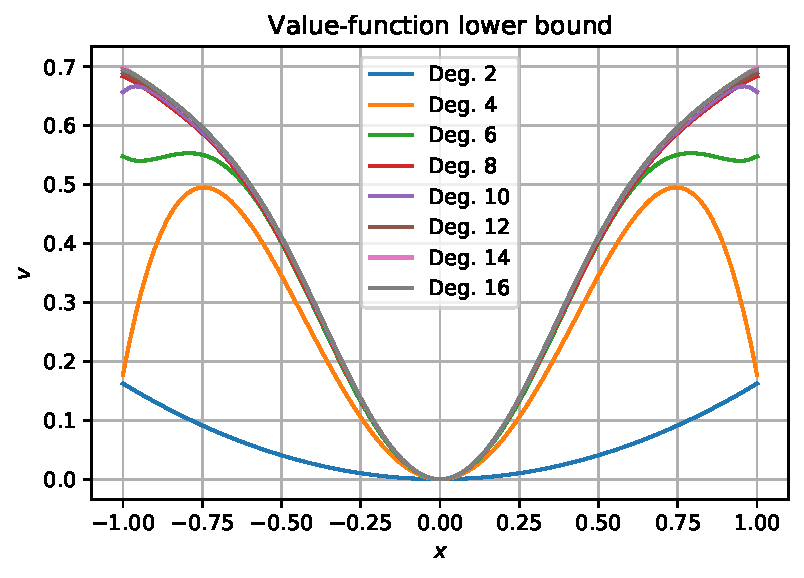
\includegraphics[width=\columnwidth]{figures/approximate_dp_scalar.pdf}
	\end{figure}
\end{columns}
\end{frame}

\begin{frame}{Pendulum swing up
\href{https://colab.research.google.com/github/TobiaMarcucci/optimal_control_pisa/blob/master/demos/pendulum_swing_up.ipynb}{\beamergotobutton{Try this in Drake}}}
\begin{columns}
	\column{.5\textwidth}
	\begin{itemize}
		\item
		Find a controller that stabilizes the pendulum in the upright configuration
		\item
		Use S-procedure to handle sines and cosines
		\item
		Approximate value function of degree 10
	\end{itemize}
	\column{.2\textwidth}
	\begin{figure}
		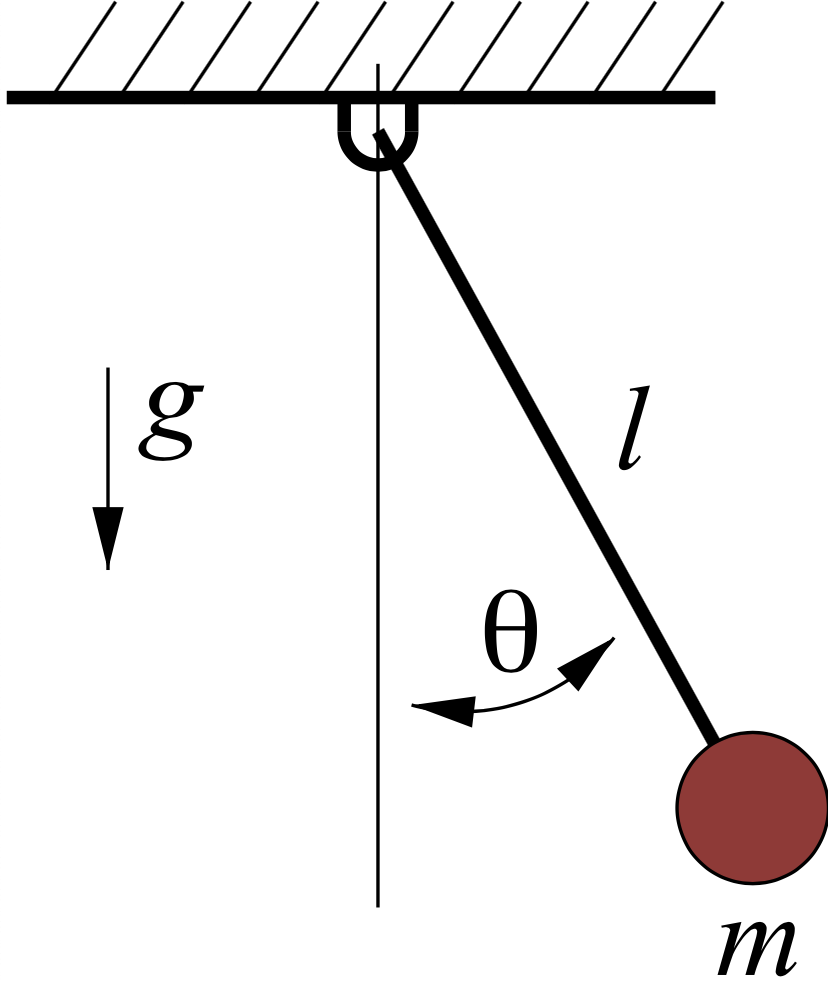
\includegraphics[width=\columnwidth]{figures/simple_pend.png}
	\end{figure}
\end{columns}
\end{frame}

\section{Conclusions}
\begin{frame}
	\huge
	\centering
	{\color{darkred} Conclusions}
\end{frame}

\begin{frame}{Take-home messages}
\begin{itemize}
\item
Convex optimization is a mature and extremely powerful tool
\item
Not all the convex optimizations are easy
\item
Semidefinite programs are easy and they can tackle surprisingly many problems
\item
Sums-of-squares optimization is a game changer in stability analysis
\item
SOS is quite effective also in optimal control
\end{itemize}
\end{frame}

\section{Bibliography}
\begin{frame}
	\huge
	\centering
	{\color{darkred} Bibliography}
\end{frame}

\begin{frame}
\footnotesize
Software:
\begin{itemize}
\item
Drake - \href{https://drake.mit.edu}{{\color{blue}https://drake.mit.edu}}
\end{itemize}
Convex optimization:
\begin{itemize}
\item
Boyd, Vandenberghe - ``Convex Optimization''
\end{itemize}
Semidefinite programming:
\begin{itemize}
\item
Vandenberghe, Boyd - ``Semidefinite programming''
\item
Boyd, Vandenberghe - ``Convex Optimization''
\end{itemize}
Sums-of-Squares optimization:
\begin{itemize}
\item
Parrilo - ``Structured semidefinite programs and semialgebraic geometry methods in robustness and optimization''
\item
Blekherman, Parrilo, Thomas - ``Semidefinite Optimization and Convex Algebraic Geometry''
\end{itemize}
Stability theory:
\begin{itemize}
\item
Khalil - ``Nonlinear Systems''
\item
Slotine, Li - ``Applied nonlinear control''
\end{itemize}
\end{frame}

\begin{frame}
\footnotesize
Dynamic programming:
\begin{itemize}
\item
Bertsekas - ``Dynamic Programming and Optimal Control, Volume 1''
\item
Kirk - ``Optimal Control Theory an Introduction''
\item
Bressan, Piccoli - ``Introduction to the Mathematical Theory of Control''
\end{itemize}
Hamilton-Jacobi-Bellman equation:
\begin{itemize}
\item
Evans - ``Partial Differential Equations''
\end{itemize}
Approximate dynamic programming:
\begin{itemize}
\item
Bertsekas - ``Dynamic Programming and Optimal Control, Volume 2''
\item
De Farias, Van Roy - ``The linear programming approach to approximate dynamic programming''
\item
Lasserre et al. - ``Nonlinear optimal control via occupation measures and LMI-relaxations''
\item
Wang, Boyd - ``Approximate dynamic programming via iterated Bellman inequalities''
\item
Other works from Lygeros' group, e.g. Summers et al. - ``Approximate Dynamic Programming via Sum of Squares Programming''
\end{itemize}
\end{frame}

\end{document}